% 非互換なパッケージに自動でパッチを当てる
% https://qiita.com/wtsnjp/items/76557b1598445a1fc9da
\RequirePackage{plautopatch}
% pdfpagesの依存パッケージのエラー回避
% https://okumuralab.org/tex/mod/forum/discuss.php?d=2956
% https://github.com/aminophen/gentombow/issues/9
\plautopatchdisable{eso-pic}
% documentclassでdvipdfmx指定をするので個別パッケージでのドライバ指定は不要
% https://qiita.com/Aruneko/items/13e015bce0112143f277
\documentclass[autodetect-engine, dvi=dvipdfmx, 10pt, a4paper, ja=standard]{bxjsarticle}

% 印刷時の用紙サイズ設定
\usepackage{bxpapersize}% これでOK!

% pdf-version
\usepackage[1.4]{bxpdfver}

% 日本語環境での字体修正
\usepackage{otf}
% フォントエンコーディングの名前をオプションで指定する
\usepackage[T1]{fontenc}
\usepackage{lmodern}% Latin Modern フォントを使う

% graphicx
\usepackage{graphicx}
\usepackage{grffile}% include graphicsの画像ファイル名の制限を撤廃

% \begin{comment} ... \end{comment} で複数行コメントアウト
\usepackage{comment}

% 数学系 インライン数式を \[ \] と書く癖をつける
\usepackage{amsmath,amssymb,amsthm}
\usepackage{amsfonts}
\usepackage{mathtools}
\usepackage{bm} % bold math

% 化学
\usepackage[version=4]{mhchem}

% SI単位系
\usepackage{siunitx}

% 表関連
\usepackage{multirow} % 表のセルの結合
\usepackage{booktabs} % 表の線がすごくなる. Table Generatorを使うときはbooktabsモードにする
\usepackage{caption} % キャプションをいじる
\usepackage{float} % 図表を絶対にそこに置く確固たる意思

% その他便利な子
\usepackage{pdfpages} % pdfを挿入
\usepackage[hyphens]{url} % urlをきれいに表示する
\usepackage{ulem} % 下線を強化
\usepackage[at]{easylist} % @をつかって箇条書き
% \usepackage{minted}
% \usepackage{termsim} % ターミナルを再現...誰得?

% ハイパーリンクを生成
% sectionなどで数式を使う場合は \texorpdfstring{texstring}{pdfstring}をする
\usepackage{hyperref}
\usepackage{pxjahyper}
\usepackage{footnotebackref} % 脚注から本文へ飛べる


% ここからはソースコードを表示する設定
\usepackage{listings, plistings, color}
\renewcommand{\lstlistingname}{Code}
\definecolor{OliveGreen}{rgb}{0.0,0.6,0.0}
\definecolor{Orenge}{rgb}{0.89,0.55,0}
\definecolor{SkyBlue}{rgb}{0.28, 0.28, 0.95}
\lstset{
    language={Ruby}, % 言語の指定
    basicstyle={\ttfamily},
    identifierstyle={\small},
    commentstyle={\smallitshape},
    keywordstyle={\small\bfseries},
    ndkeywordstyle={\small},
    stringstyle={\small\ttfamily},
    frame={tb},
    breaklines=true,
    columns=[l]{fullflexible},
    numbers=left,
    xrightmargin=0zw,
    xleftmargin=3zw,
    numberstyle={\scriptsize},
    stepnumber=1,
    numbersep=1zw,
    lineskip=-0.5ex,
    stepnumber=1,       % 行数の増間
    numbersep=1zw,      % 行数の余白
    xrightmargin=0zw,   % 左の余白
    xleftmargin=2zw,    % 右の余白
    framexleftmargin=18pt,  % フレームからの左の余白
    keepspaces=true,    % スペースを省略せず保持
    lineskip=-0.2ex,    % 枠線の途切れ防止
    tabsize = 4,        % タブ数
    showstringspaces=false,  %文字列中の半角スペースを表示させない
    keywordstyle={\color{SkyBlue}},     %キーワード(int, ifなど)の書体指定
    commentstyle={\color{OliveGreen}},  %注釈の書体
    stringstyle=\color{Orenge}          %文字列
}

% \refだけで「図」や「式」を自動挿入
% https://zenn.dev/arks/articles/3697b25d03f8a8
% subfigureが文書にあると小節を参照する際に使う\subrefがおかしくなるので注意
%% increase link area for cross-references and autoname them, [130514]
\AtBeginDocument{\renewcommand{\ref}[1]{\mbox{\autoref{#1}}}}

\def\equationautorefname~#1\null{式(#1)\null}
\def\figureautorefname~#1\null{図#1\null}
\def\subfigureautorefname#1\null{図#1\null}
\def\tableautorefname~#1{表#1}
\def\lstlistingautorefname~#1{コード#1}

\def\partautorefname#1\null{第#1部\null}
\def\chapterautorefname#1\null{第#1章\null}
\def\sectionautorefname#1\null{#1節}
\def\subsectionautorefname~#1\null{#1節}
\def\subsubsectionautorefname#1\null{#1節}
\def\paragraphautorefname#1\null{#1段落}
\def\subparagraphautorefname#1\null{#1段落}

\def\Itemautorefname#1\null{項目#1\null}
\def\Hfootnoteautorefname#1\null{脚注#1\null}
\def\theoremautorefname#1\null{定理#1\null}
\def\FancyVerbLineautorefname#1\null{#1行\null}
% \def\pageautorefname#1\null{ページ#1\null}
\def\appendixautorefname#1\null{付録#1\null}


\title{MICS実験第一 J1課題レポート}
\author{学籍番号 2210342, 鈴木謙太郎}
\date{\today}
\begin{document}
\maketitle


% \bibliography{hoge} %hoge.bibから拡張子を外した名前
% \bibliographystyle{junsrt} %参考文献出力スタイル
% 使用する際は latex-workshop.latex.recipe.default を
% ptex2pdf (uplatex) → bibtex → ptex2pdf (uplatex) × 2
% に変更

\section{問題1}

\subsection{目的}

本問題では,FPGAにおいて入出力を接続する方法について理解することを目指す.


\subsection{原理・理論}

本問に限らずこの実験において用いるFPGAとは,Field Programmable Gate Arrayの略であり,
プログラムによって自由に書き換えられる論理素子である.

本実験では「Quartus」と呼ばれるソフトウェアを用いてGUI上で回路を設計し,
その回路をFPGAに書き込むことで,実際にハードウェア上で回路を動作させることができる.

実際に回路を構成する際は,入力ピン(ボタンやスイッチ,クロック信号など)と出力ピン(LEDなど)の間に
組み合わせ回路などを配置し,それらを接続することで入力に対して出力を得ることができる.

\subsection{回路のアルゴリズム・設計}

本問では,実験資料で示されたように,FPGAボード上のトグルスイッチや押しボタンスイッチに対して
LEDを接続することで,入力が与えられた際にLEDが点灯するような回路を設計する.

\subsection{実際に設計した回路}

\ref{fig:ex1}のような回路を設計した.

単純に入力スイッチのピンと出力LEDのピンを接続することで,
スイッチの入力がLEDの出力に反映されるようになっている.


\begin{figure}[htbp]
	\centering
	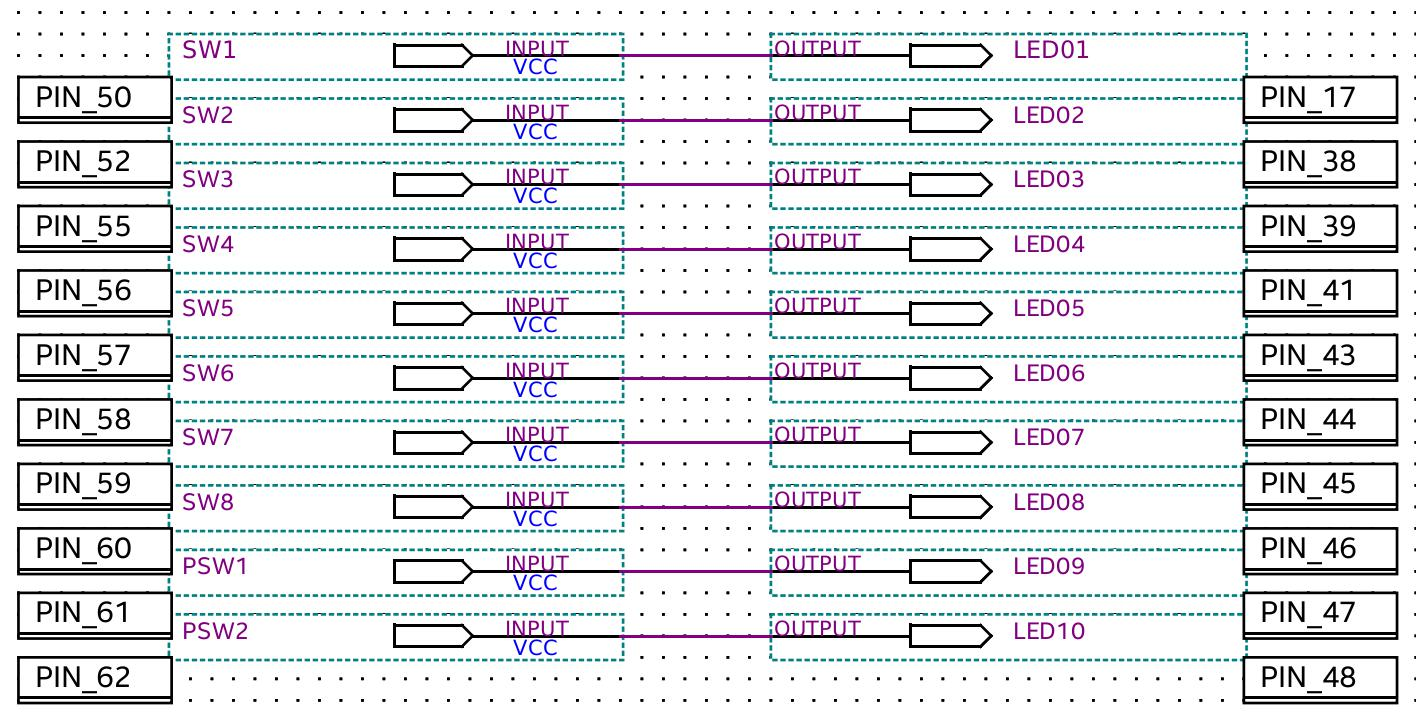
\includegraphics[width=\columnwidth]{asset/ex1-トリミング.jpg}
	\caption{問題1で設計した回路}
	\label{fig:ex1}
\end{figure}


\subsection{実験・測定結果}

実際にFPGAボードに書き込んだ結果,スイッチを操作することでLEDが点灯することが確認できた.

\ref{fig:ex1}からも分かる通り,この回路では各スイッチの入力は独立しているので,
同時に複数のスイッチを操作しても出力が変化することはなかった.

\section{問題2}

\subsection{目的}

本問では,ANDゲート,ORゲート,NOTゲートをはじめとするゲート回路を
FPGA上で動作させることを通じて,組み合わせ回路の設計方法を理解することを目指す.

組み合わせ回路とは,入力に対して出力が一意に定まる回路のことである.
この回路は,ゲート(AND,OR,NOTなど)のみを組み合わせることで構成される.

\subsection{仕様}
本問では,2ビットの入力$x = x_1 x_0$と$y = y_1 y_0$に対して,
$x > y$のとき出力$z = 1$,それ以外のとき$z = 0$となる回路を設計する.
なお,これらの入力は符号なしの2進数として扱うものとする.

\subsection{回路のアルゴリズム・設計}

このような回路を作るにあたって,真理値表やカルノー図を用いることで
簡略化された効率のよい論理回路を作ることができる.

本問でも\ref{fig:ex2-karnaugh}のような真理値表とカルノー図を用いることで,
出力$z$の論理式を\ref{eq:ex2}のように求めた.

\begin{equation}
	\label{eq:ex2}
	z = x_0 y_1' y_0' + x_1 x_0 y_0' + x_1 y_1'
\end{equation}



\begin{figure}[htbp]
	\centering
	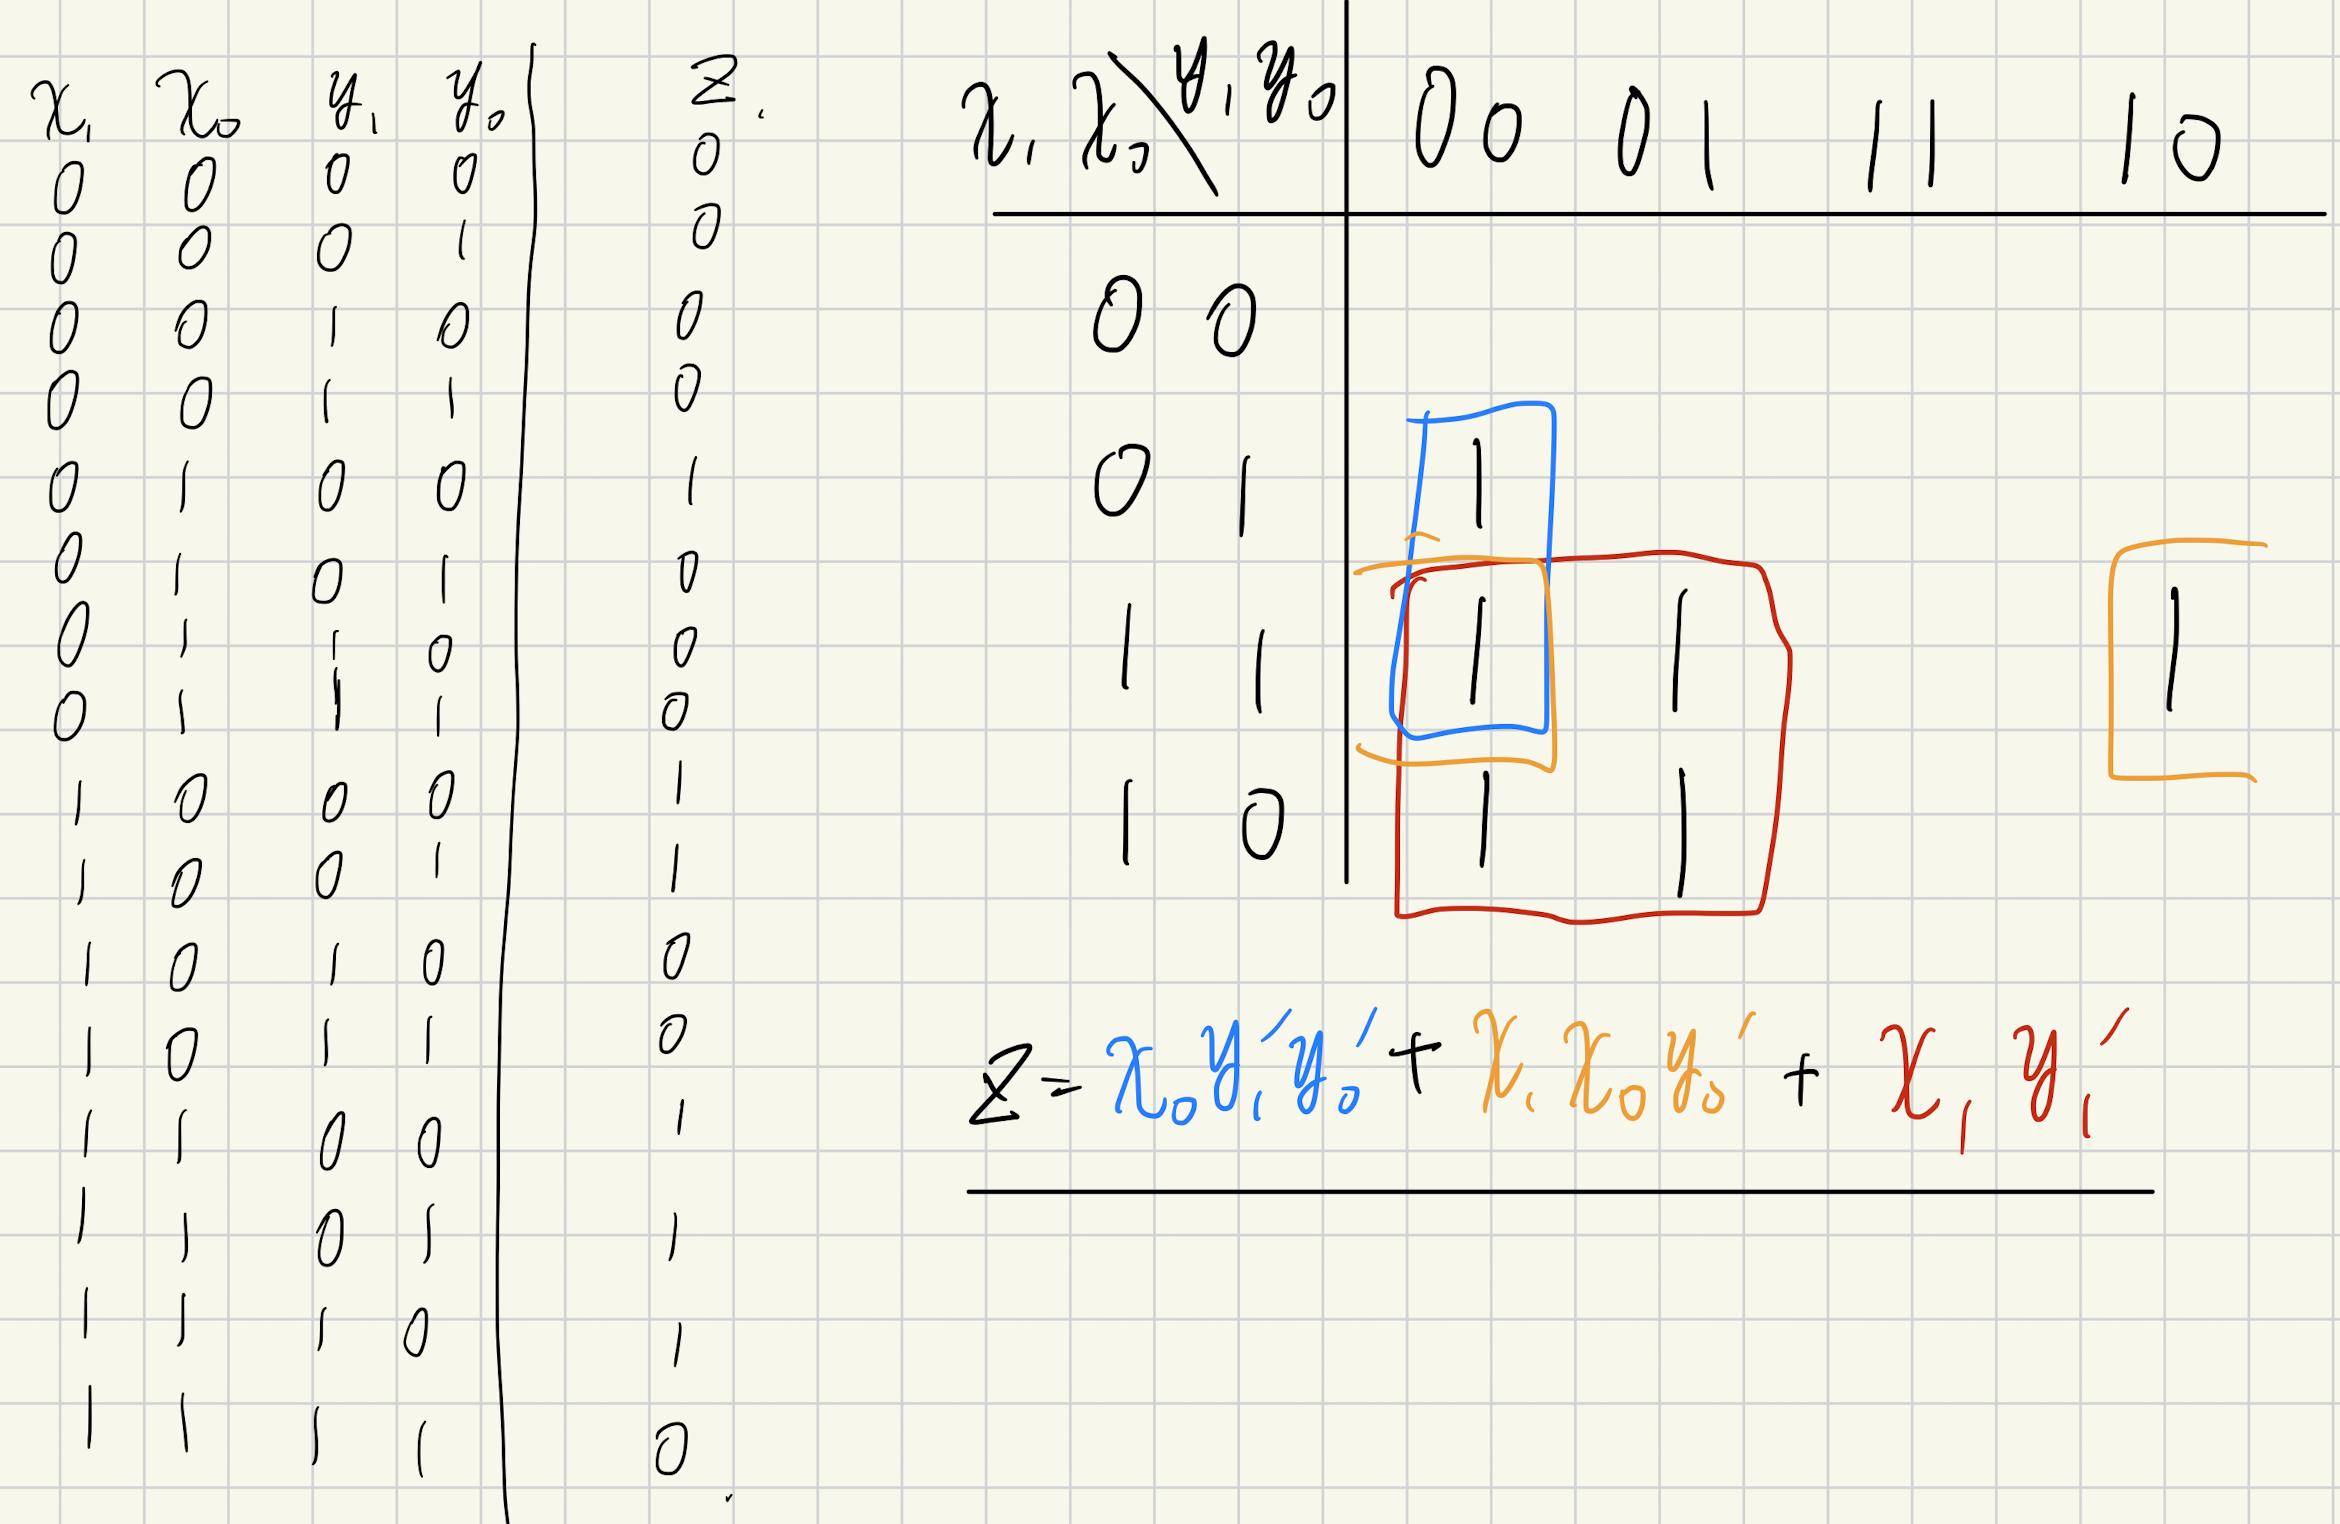
\includegraphics[width=0.8\columnwidth]{asset/ex2_fig.png}
	\caption{問題2で用いた真理値表とカルノー図}
	\label{fig:ex2-karnaugh}
\end{figure}


実際の回路設計では,\ref{eq:ex2}の論理式をそのままゲートによる組み合わせ回路に変換することで,
期待する出力を得ることが可能である.
また,入力にはすべてトグルスイッチを用いた.

\subsection{実際に設計した回路}

\ref{eq:ex2}をもとに,\ref{fig:ex2}のような回路を設計した.

\begin{figure}[htbp]
	\centering
	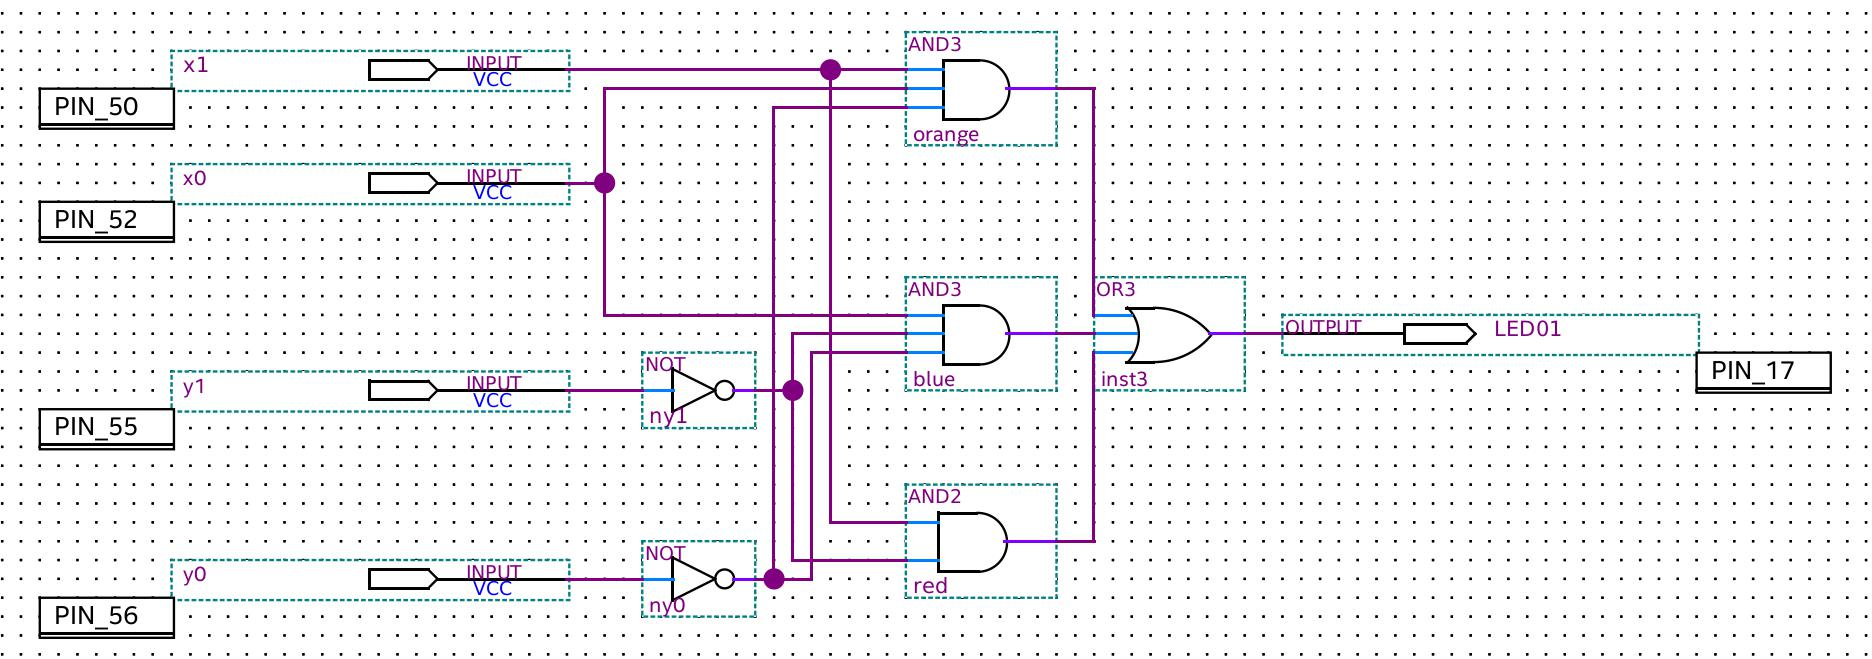
\includegraphics[width=\columnwidth]{asset/ex2_trim.jpg}
	\caption{問題2で設計した回路}
	\label{fig:ex2}
\end{figure}

\subsection{実験・測定結果}

実際にFPGAボードに書き込んだ結果,$x > y$のときに限りLEDが点灯し,$x = y$や$x < y$となるときは消灯することが確認できた.
よって,期待する出力を得ることができていると考えられる.

\section{問題3}
\label{sec:ex3}

\subsection{目的}
本問では,D型フリップフロップを用いた微分回路を設計することで,順序回路の設計方法を理解することを目指す.

\subsection{原理・理論}
順序回路とは,組み合わせ回路とは異なり,出力が入力だけでなく過去の状態にも依存する回路のことである.
このような回路は,フリップフロップなどの記憶素子を用いることで設計することができる.

フリップフロップは,1ビットので0田を記憶できる素子である.特にD型フリップフロップは,
データとクロック信号を入力として受け取り,クロックが立ち上がるときにD入力の値を出力に反映する.
このような性質上,クロックはフリップフロップの動作を制御するために必要である.
この入力を人の手で正確に切り替えることは難しいため,FPGAボードに備え付けられたクロック信号発生器を用いる.

本問で作成する微分回路とは,入力信号の立ち上がりエッジを検出し,そのエッジが立ち上がるたびに出力信号をトグルする回路である.
このような回路を作成することで,人間がスイッチを1回押したときに,1クロックの長さのパルスを1回だけ出力することができる.

\subsection{回路のアルゴリズム・設計}

本問では,クロック信号を入力として受け取り,その立ち上がりエッジを検出する微分回路を設計する.

フリップフロップなどを含む順序回路を設計する際には,出力が過去の状態に依存するため,
状態遷移図などを作成して設計を行うことが一般的である.

\ref{fig:ex3}のような回路を設計するにあたって,
便宜上左側のD型フリップフロップの入力を$D_0$, 出力を$Q_0$とし,
右側のD型フリップフロップの入力を$D_1$, 出力を$Q_1$とする.

\begin{figure}[htbp]
	\centering
	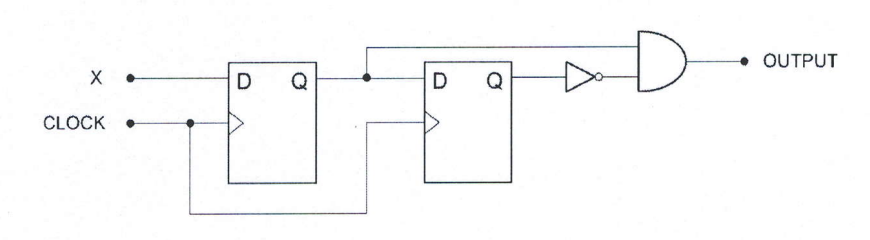
\includegraphics[width=\columnwidth]{asset/ex3_notebook.png}
	\caption{問題3で設計する微分回路の回路図(実験資料より引用)}
	\label{fig:ex3}
\end{figure}

この回路の真理値表は\ref{fig:ex3-tf}のようになった.

\begin{figure}[H]
	\centering
	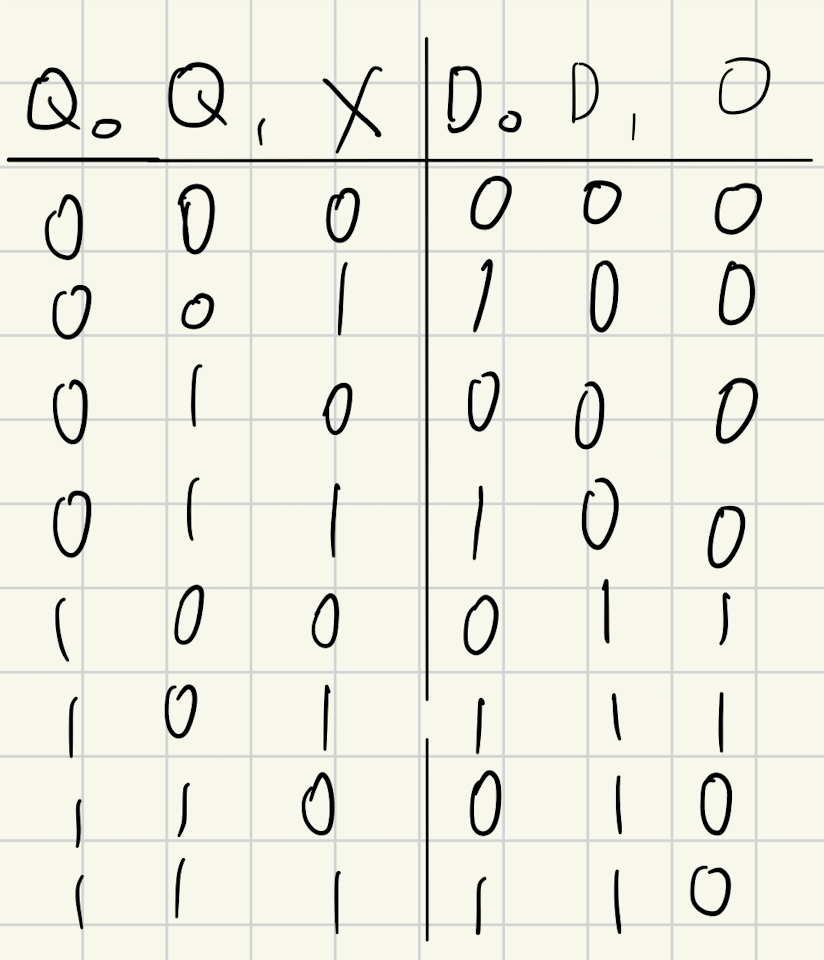
\includegraphics[width=0.8\columnwidth]{asset/ex3_tf.png}
	\caption{問題3で用いた真理値表}
	\label{fig:ex3-tf}
\end{figure}

これの真理値表をもとに,\ref{fig:ex3-state}のような状態遷移図を作成した.

\begin{figure}[H]
	\centering
	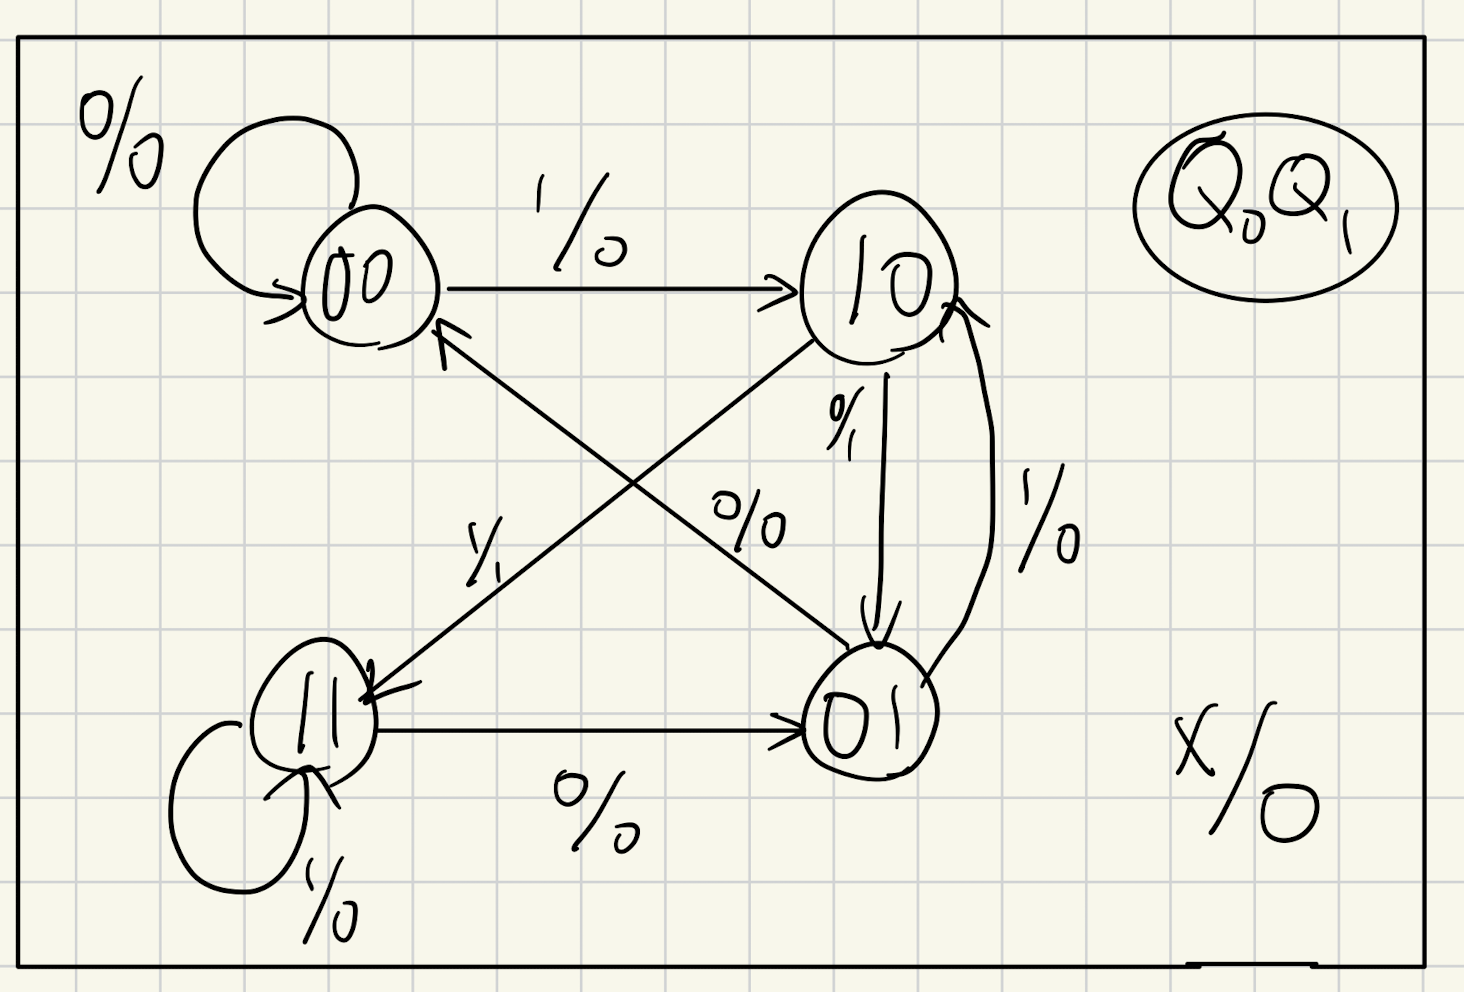
\includegraphics[width=0.8\columnwidth]{asset/ex3_state.png}
	\caption{問題3で用いた状態遷移図}
	\label{fig:ex3-state}
\end{figure}

ここで,状態00と状態01に注目すると,ともに0を入力すると0を出力して状態00に遷移し,
1を入力すると1を出力して状態10に遷移することが分かる.よって,この2つの状態は同じものとみなせる.

このような同じ状態が複数ある場合,その状態への遷移とその状態からの遷移をまとめることで,
状態遷移図を\ref{fig:ex3-state-refine}のように簡略化することができる.

\begin{figure}[H]
	\centering
	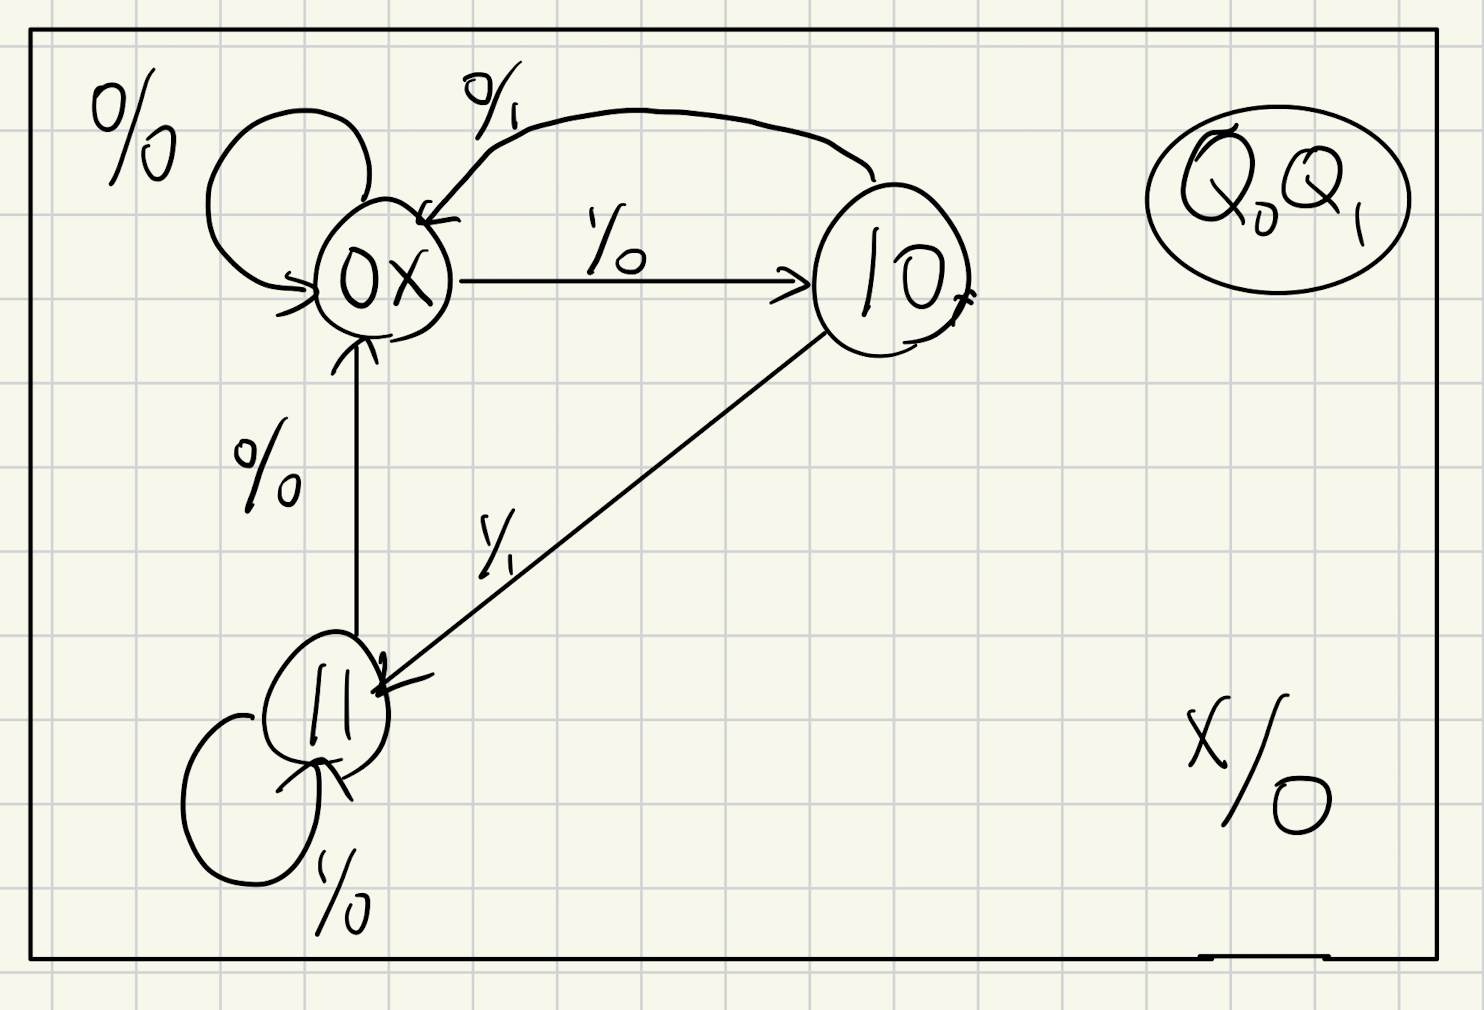
\includegraphics[width=0.8\columnwidth]{asset/ex3_state_refine.png}
	\caption{\ref{fig:ex3-state}を簡略化した後の状態遷移図}
	\label{fig:ex3-state-refine}
\end{figure}

\subsection{実際に設計した回路}

\ref{fig:ex3}の回路を,実験資料で示された2ビットカウンタ回路と接続し,
\ref{fig:ex3-cropped}のような回路を設計した.
これをQuartusのRTL Viewerで図持すると\ref{fig:ex3-rtl}のようになる.

\begin{figure}[H]
	\centering
	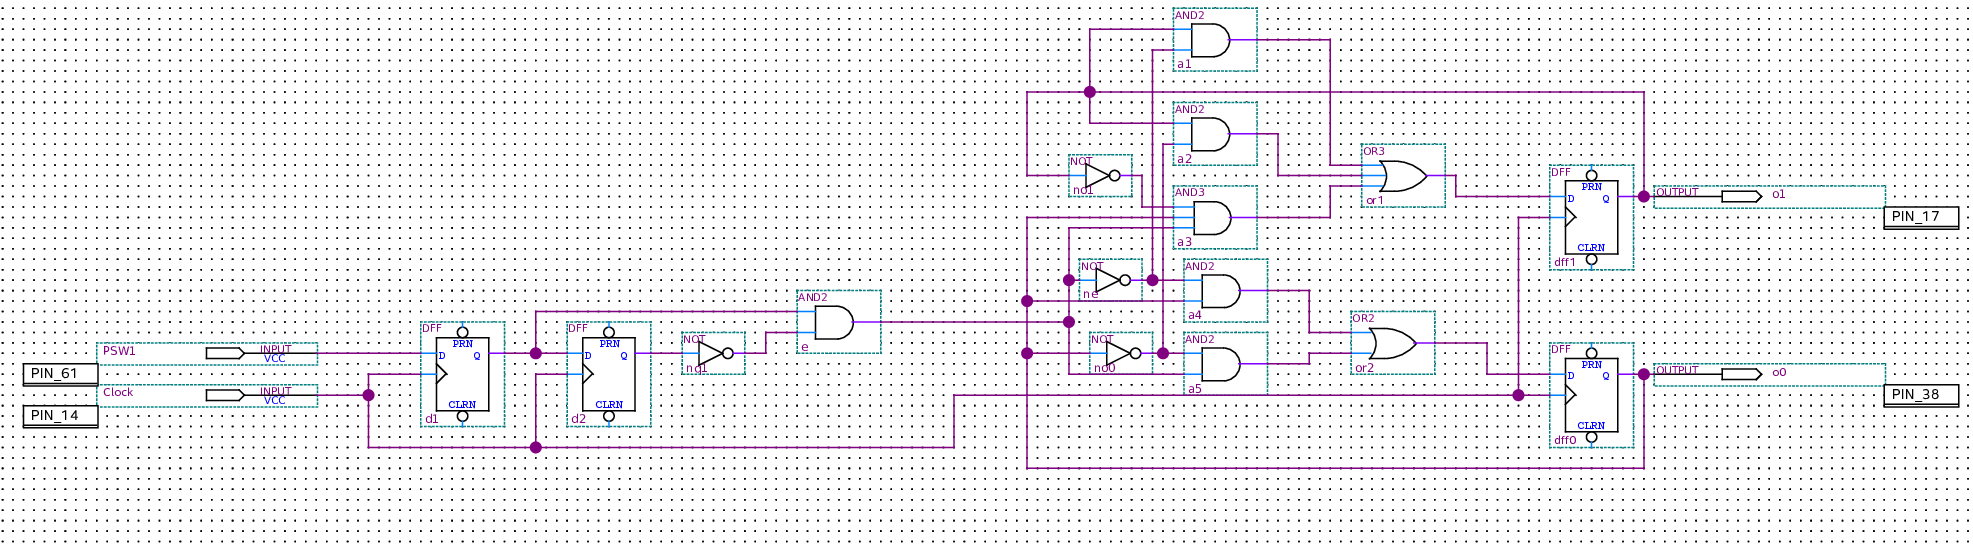
\includegraphics[width=\columnwidth]{asset/ex3.png}
	\caption{問題3で設計した回路}
	\label{fig:ex3-cropped}
\end{figure}

\begin{figure}[H]
	\centering
	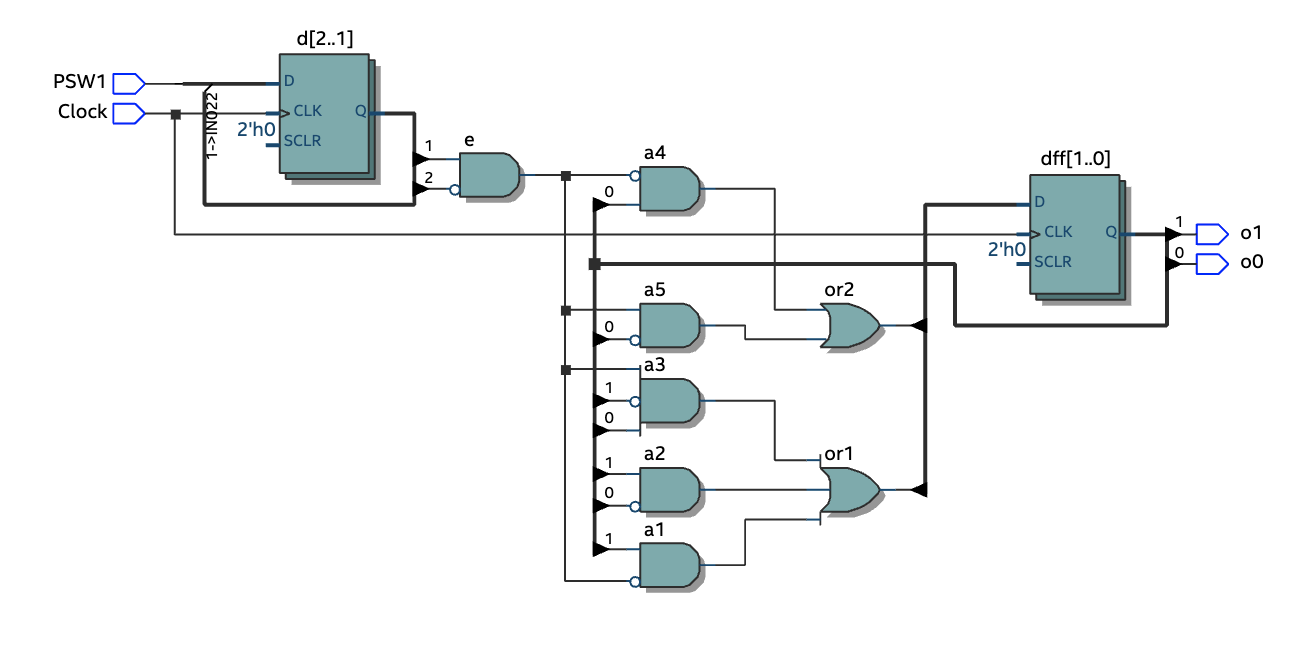
\includegraphics[width=\columnwidth]{asset/ex3_pretty.png}
	\caption{\ref{fig:ex3-cropped}をRTL Viewerで表示したもの}
	\label{fig:ex3-rtl}
\end{figure}

\subsection{実験・測定結果}

実際にFPGAボードに書き込み,クロック信号を入力した状態で押しボタンを用いて動作を確認した.
ボタンを押した長さにかかわらず,出力LEDに表示されるカウンタの値が1ずつ増加したので,
微分回路が正常に動作していると考えられる.

\subsection{考察}
このような微分回路を用いることで,人間がスイッチを操作したときに,1クロックの長さのパルスを1回だけ出力することができる.
状態遷移のある回路は,2クロック以上の長さの信号を入力してしまうと,1回の入力に対して複数回状態遷移が発生してしまうため
正確な動作を行うことができない.そのため,このような微分回路を用いることで,正確に回路の動作を確かめることができると考えられる.

\section{問題4}

\subsection{目的}

本問では,複数のD型フリップフロップを用いた順序回路を,効率の良い論理回路を設計し理解することを目指す.

\subsection{仕様}

本問では,100円硬貨を2個受け取ると200円の切符を出力する\ref{fig:ex4-image}のような自動販売機の制御回路Tを設計する.

\begin{figure}[H]
	\centering
	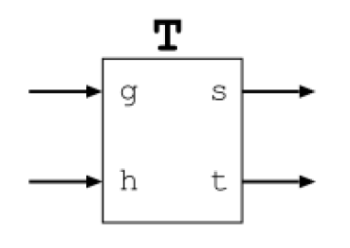
\includegraphics[width=0.8\columnwidth]{asset/ex4_image.png}
	\caption{問題4で設計する自動販売機の制御回路のイメージ(実験資料より引用)}
	\label{fig:ex4-image}
\end{figure}

実験資料で示された動作条件を下に,以下のような仕様を満たす回路を設計する.

\begin{easylist}[enumerate]
	@ 100円を入れる動作(入力$h$)をPSW1, 切符を取る動作(入力$g$)をPSW2で与える.
	@ 出力$s$をLED1, $t$をLED2で表示する.
	@ 切符が出ていない時,切符を取る動作(入力$g$)はドントケアとして扱う(出力に影響を与えない).
	@ 切符が出ている時,100円を入れる動作(入力$h$)はドントケアとして扱う(出力に影響を与えない).
\end{easylist}


\subsection{回路のアルゴリズム・設計}


仕様を元に,\ref{fig:ex4-tf}のような真理値表を作成した.
また,この真理値表をもとに\ref{fig:ex4-karnaugh}のようなカルノー図と
\ref{fig:ex4-state}のような状態遷移図を作成した.


\begin{figure}[H]
	\centering
	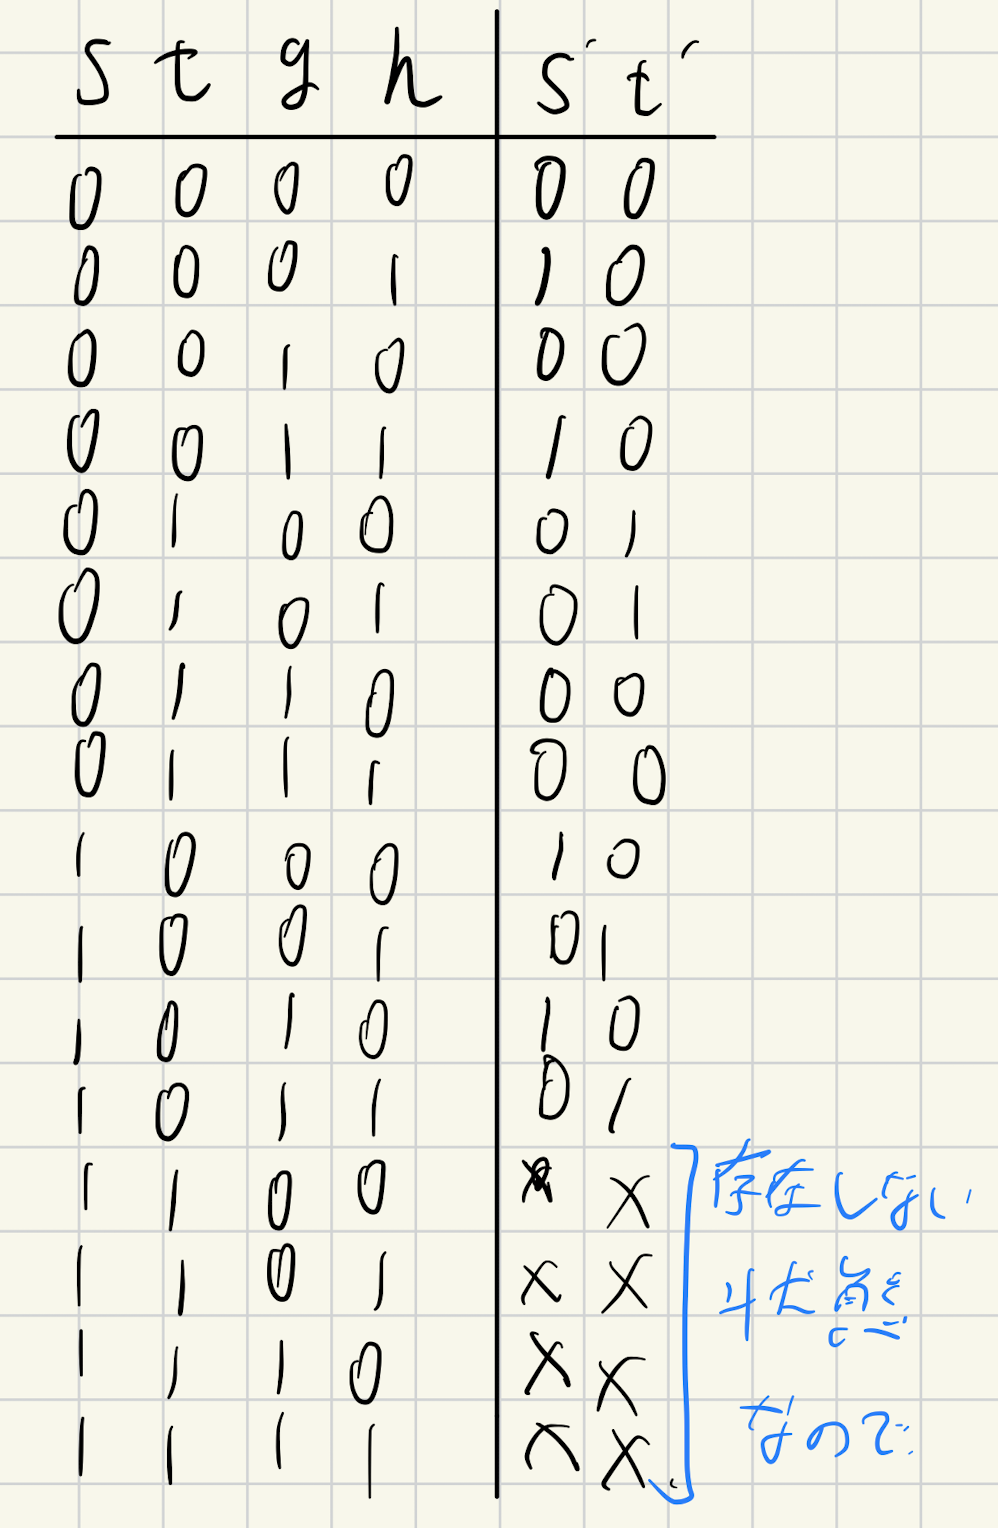
\includegraphics[width=0.8\columnwidth]{asset/ex4_tf.png}
	\caption{問題4で用いた真理値表}
	\label{fig:ex4-tf}
\end{figure}


\begin{figure}[H]
	\centering
	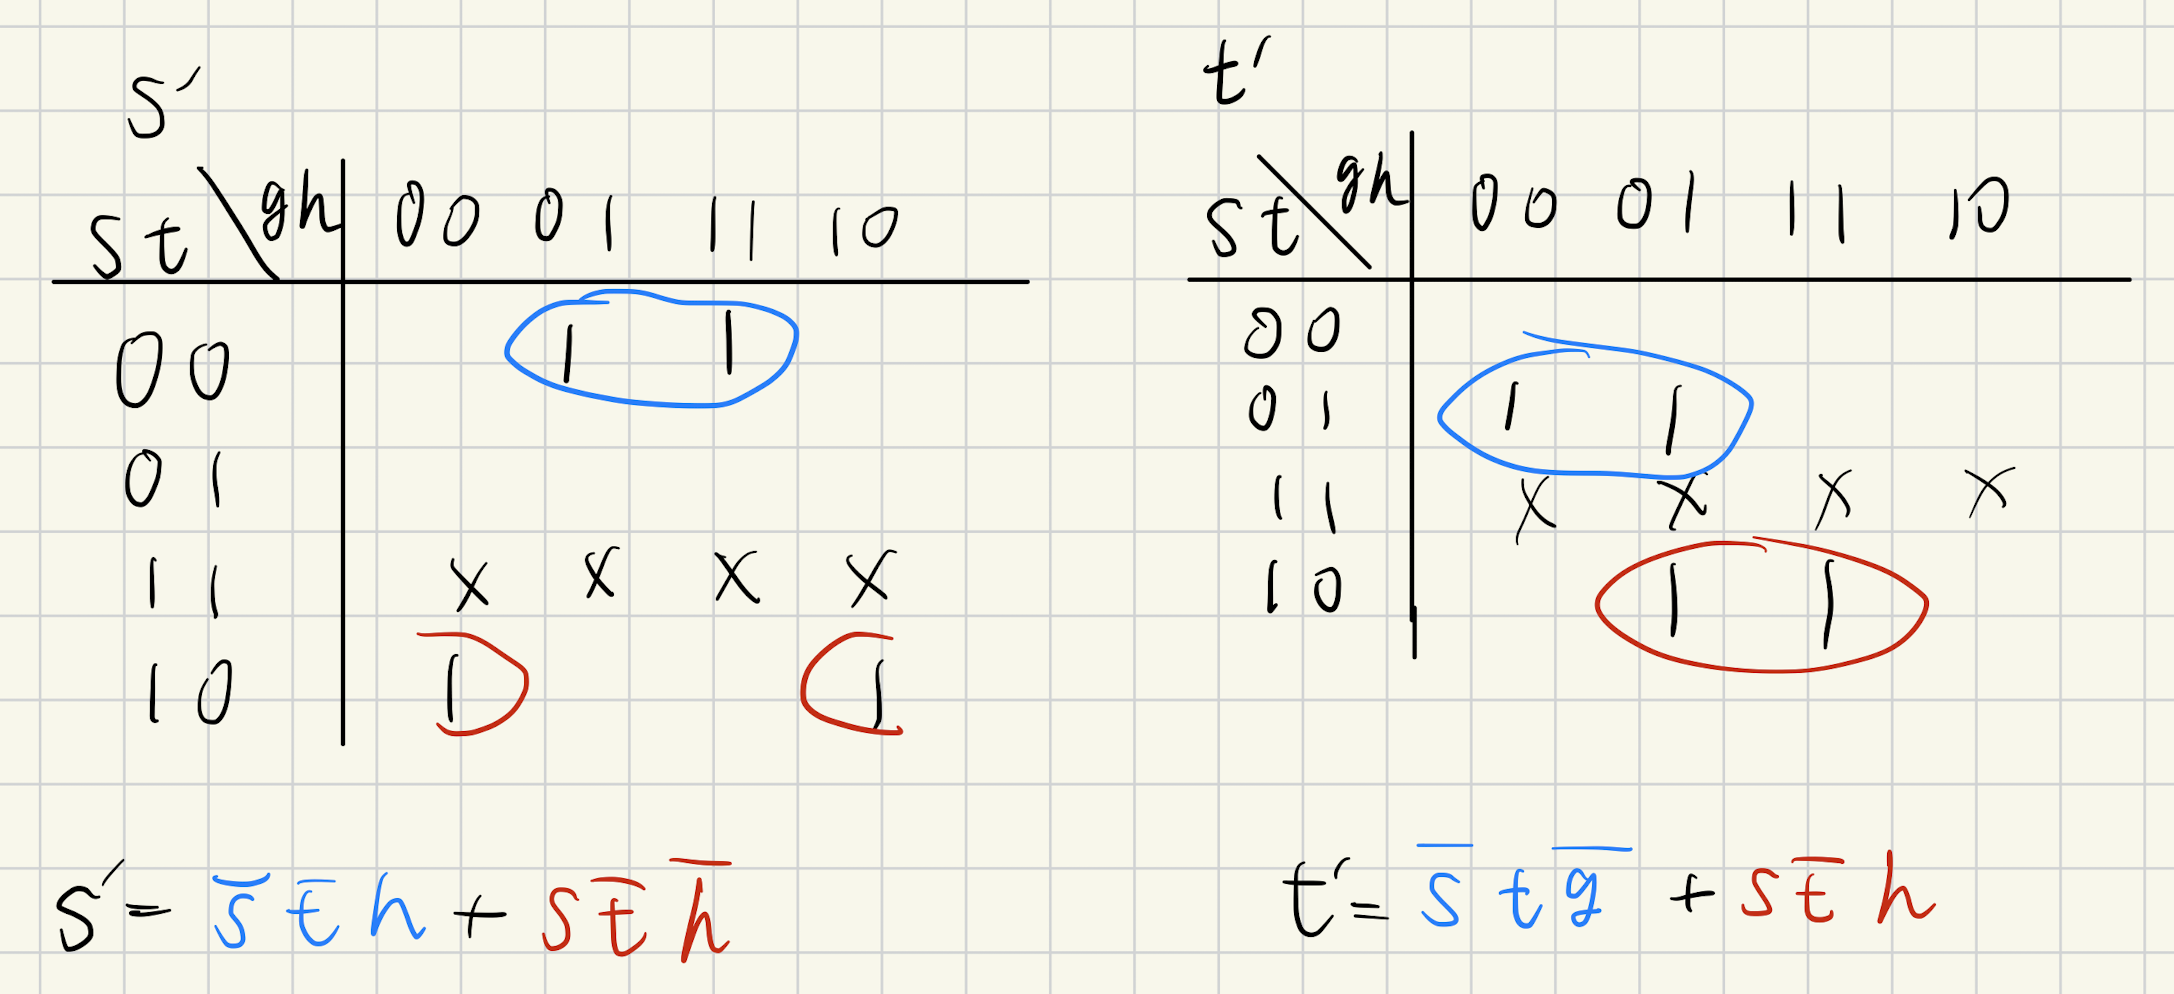
\includegraphics[width=0.8\columnwidth]{asset/ex4_ka.png}
	\caption{問題4で用いたカルノー図}
	\label{fig:ex4-karnaugh}
\end{figure}


\begin{figure}[H]
	\centering
	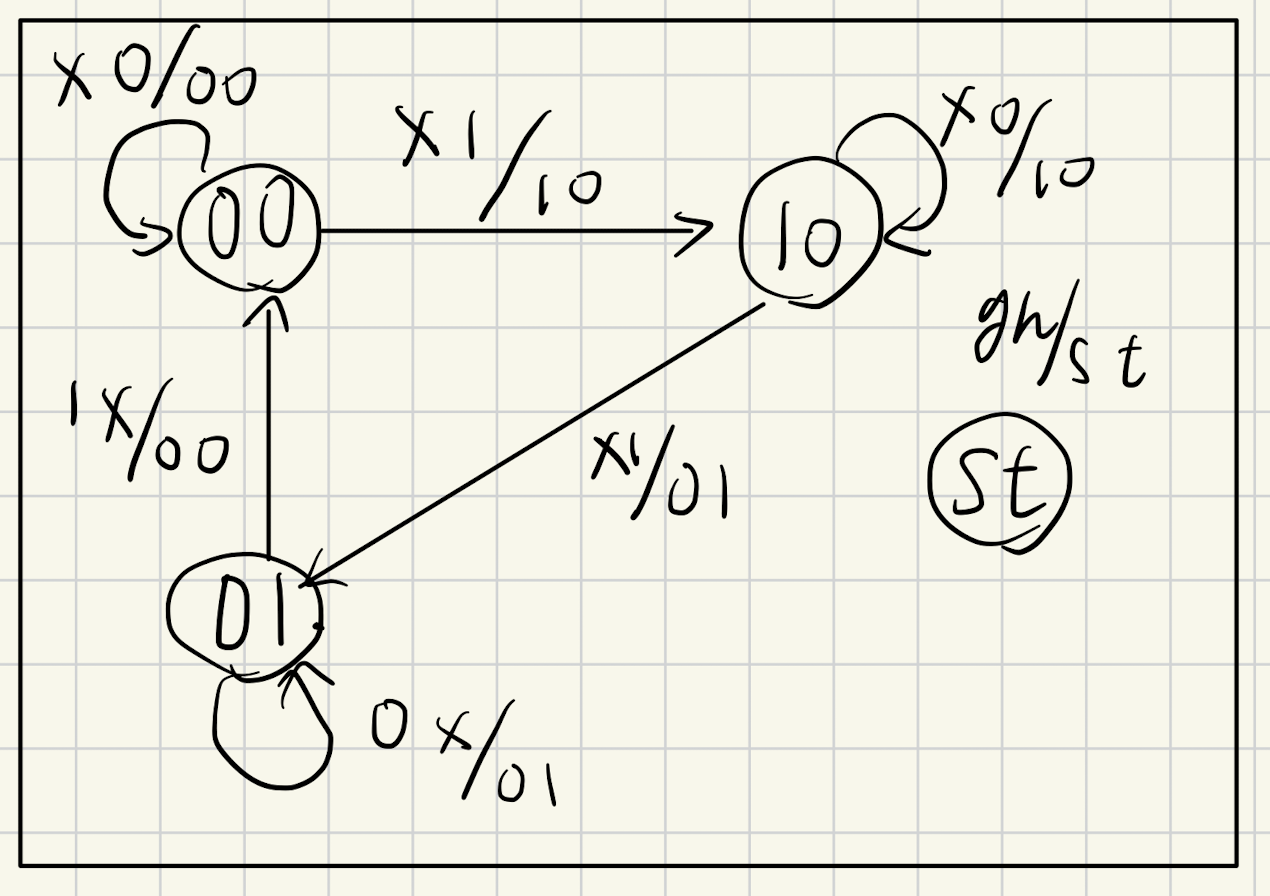
\includegraphics[width=0.8\columnwidth]{asset/ex4_state.png}
	\caption{問題4で用いた状態遷移図}
	\label{fig:ex4-state}
\end{figure}

これらの図をもとに,回路の次状態の出力$s', t'$を\ref{eq:ex4}のように求めた.

\begin{align}
	\label{eq:ex4}
	\begin{split}
		s' & = \bar{s} \bar{t} h + s \bar{t} \bar{h} \\
		t' & = \bar{s} t \bar{g} + s \bar{t} h
	\end{split}
\end{align}

\subsection{実際に設計した回路}

\ref{eq:ex4}をもとに,\ref{fig:ex4}のような回路を設計した.

\begin{figure}[H]
	\centering
	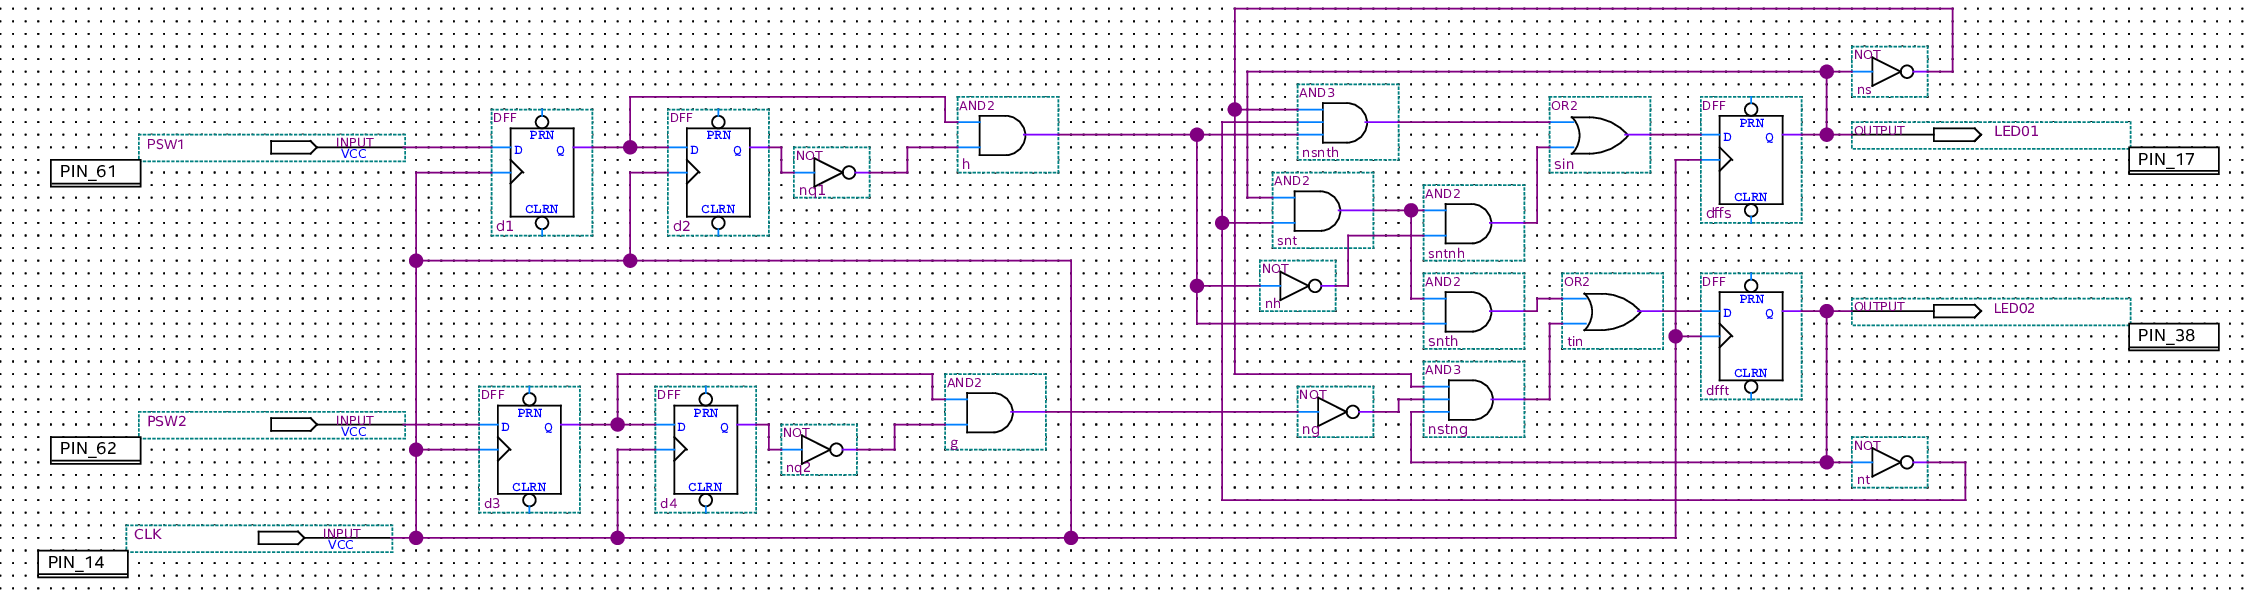
\includegraphics[width=\columnwidth]{asset/ex4.png}
	\caption{問題4で設計した回路}
	\label{fig:ex4}
\end{figure}

入力$g, h$は押しボタンを使ったうえで,\ref{sec:ex3}で扱った微分回路を用いることで
1回の操作につき1回しか状態遷移しないようにした.
それ以外の部分は,論理式をそのまま回路に変換したものである.

\subsection{実験・測定結果}
まず,2回$h$を入力した後$g$を入力する正常系の動作について,問題ないことを確認した.

次に,$h$を2回未満しか入力していない状態で$g$を入力して切符を取り出そうとしても出力が変化しないことを確認した.
また,$h$を2回入力して$g$を入力し,切符が取り出せる状態で$h$をさらに入力しても出力が変化しないことを確認した.

最後に,すべての状態において2つの入力を同時に行った場合,有効な方の入力のみが行われたように扱われることを確認した.
\ref{fig:ex4-state}からも,入力が11の場合のみ発生する遷移は存在しないため問題ないことが分かる.

以上の確認により,仕様通りの動作をすることが確認できた.

\subsection{考察}
カルノー図と論理式まであれば回路の設計を容易に行うことができるが,
その回路が正しいかを確かめる際に状態遷移図があると非常に効率的であることが分かった.

異常系を考慮した論理式や状態遷移図をもとに回路を設計することで,同時押しなどのイレギュラーな入力にも対処できるなどの堅牢性を
持たせることができるのは大変効率が良いと考えた.

\section{問題5}

\subsection{目的}

本問では,オシロスコープを用いてFPGAの動作を観察する方法を理解することを目指す.

\subsection{原理・理論}

オシロスコープは,クロック信号などの周期的な信号を波形として観測できる装置である.
周期的な信号を順序回路に入力すると,出力も周期的に変化するようになるため,このような回路の出力も観測できる.

\subsection{実験・測定結果}


\ref{fig:ex2}のような比較回路について,入力を4ビットカウントを用いた自動生成に変更した
\ref{fig:ex5}のような回路を用い,この出力をオシロスコープで観測したところ
\ref{fig:ex5-osc}のような波形が得られた.

この波形は,紫色が\ref{fig:ex5}の出力$z$で,黄色が4ビットカウンタからの出力が$0,0,0,0$に戻ったときに発されるパルス信号である.

\begin{figure}[htbp]
	\centering
	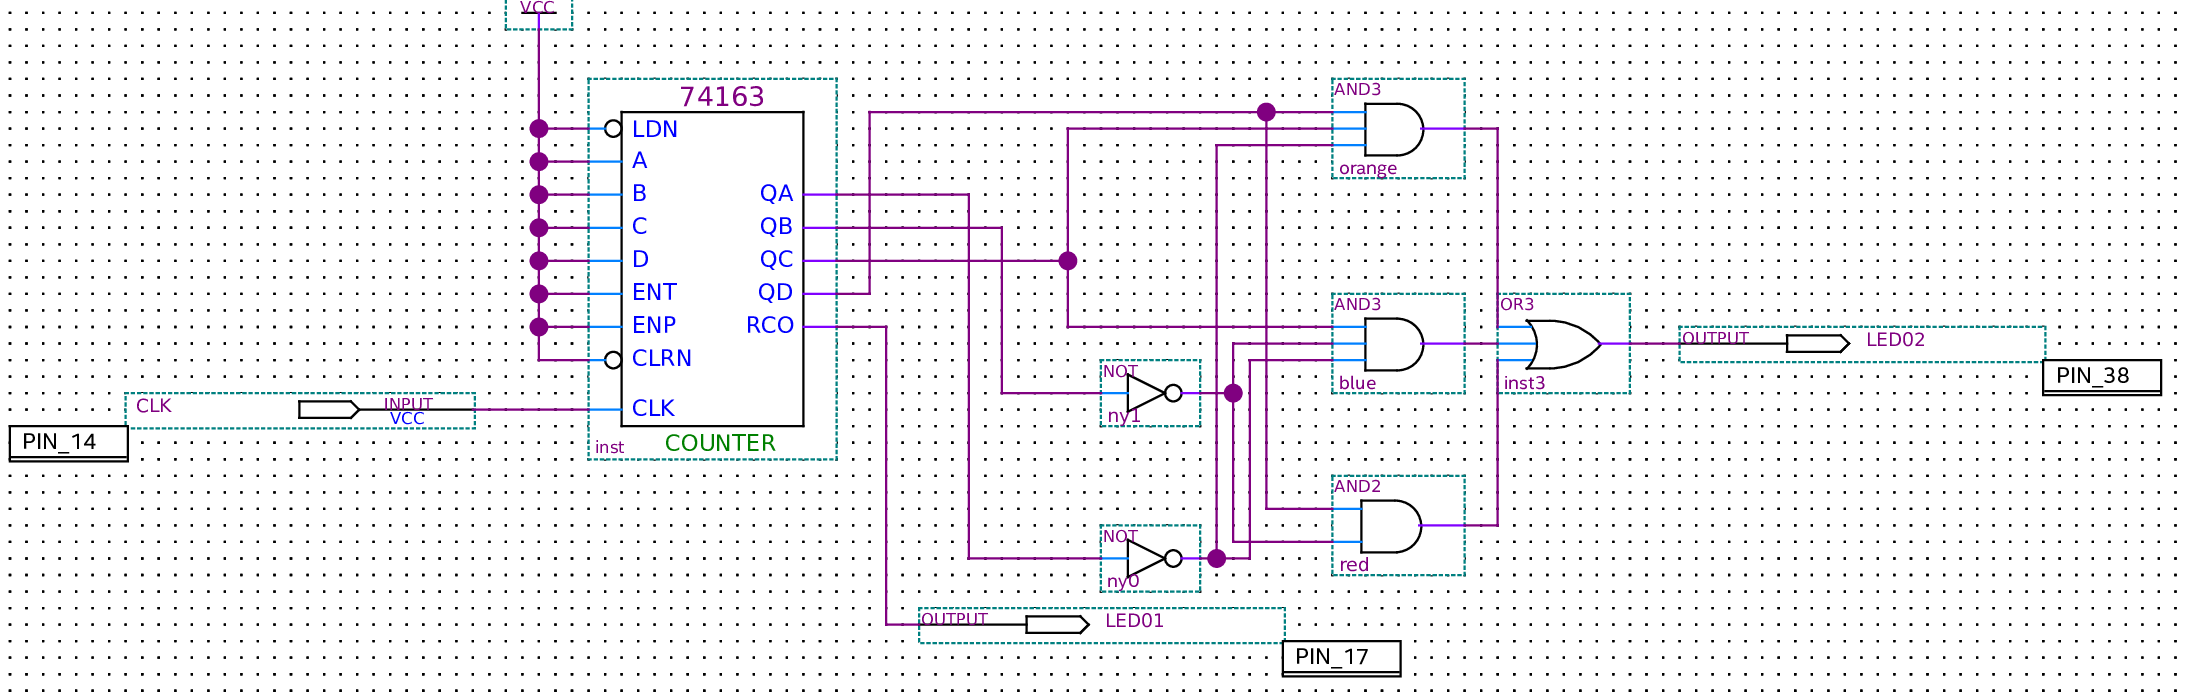
\includegraphics[width=\columnwidth]{asset/ex5.png}
	\caption{問題5で用いた回路}
	\label{fig:ex5}
\end{figure}

\begin{figure}[htbp]
	\centering
	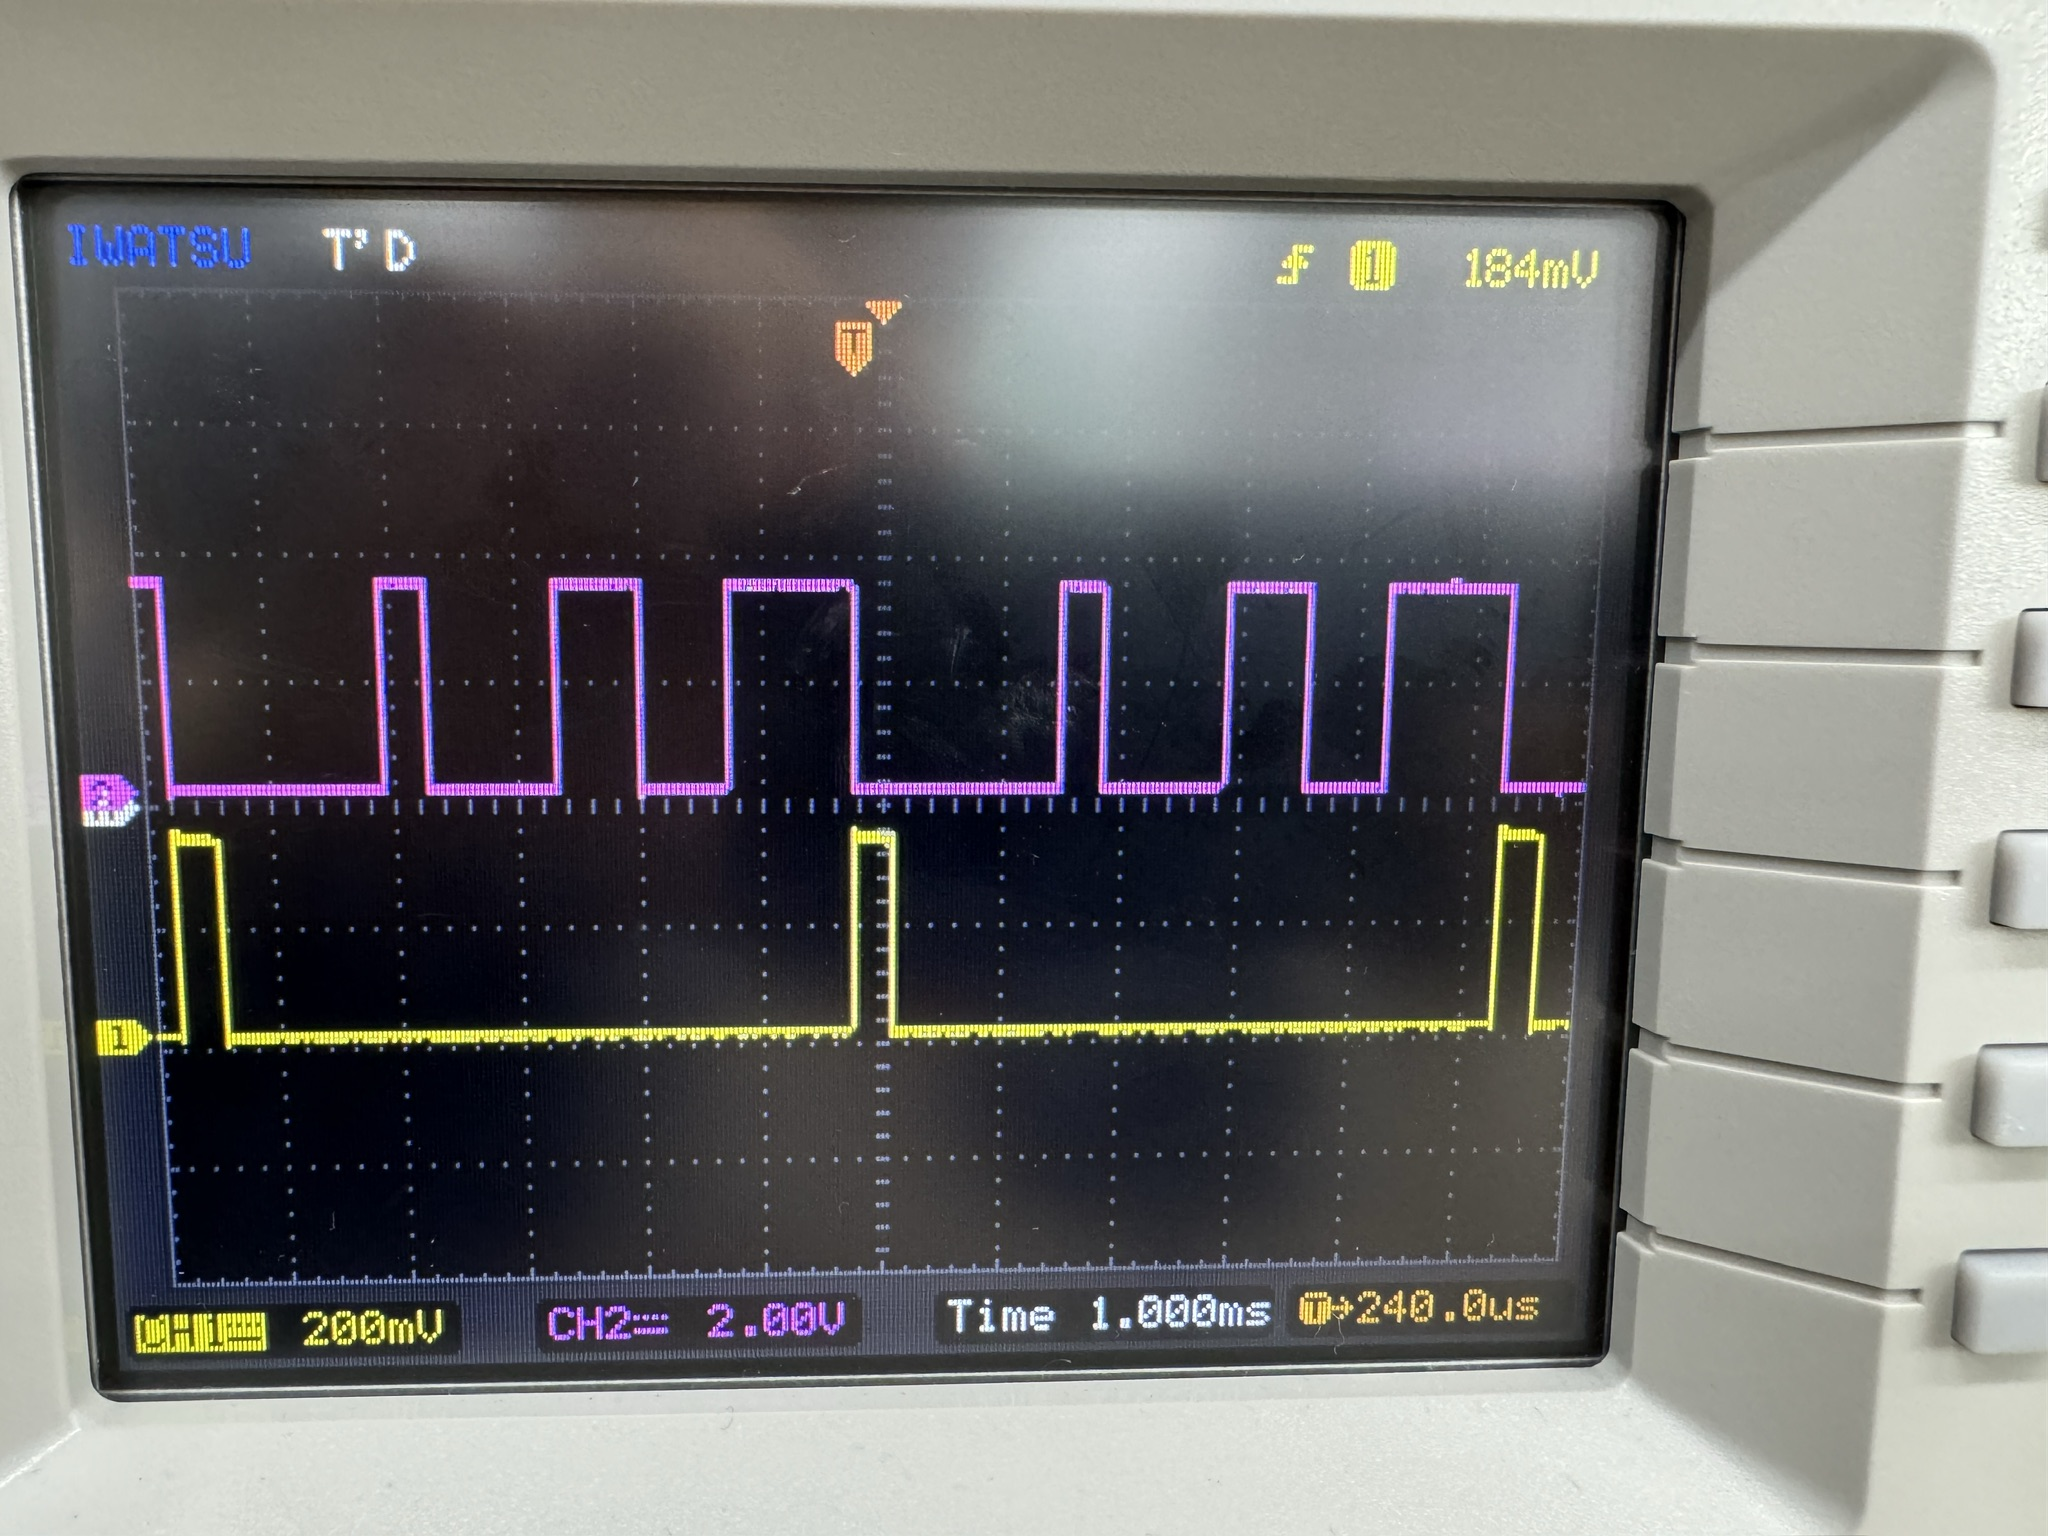
\includegraphics[width=0.8\columnwidth]{asset/ex5_wave.jpeg}
	\caption{オシロスコープで観測した波形}
	\label{fig:ex5-osc}
\end{figure}


4ビットカウンタの出力は,(QD, QC, QB, QA)を符号なし2進数として読んだときに,0から15までの値を取るように変化する.
よって,QAを$y_0$, QBを$y_1$, QCを$y_2$, QDを$y_3$とすることで,\ref{fig:ex2-karnaugh}の真理値表を見たときに
上から下へと入出力が変化することになる.

これを踏まえて\ref{fig:ex2-karnaugh}の$z$と\ref{fig:ex5-osc}の紫色の波形を見比べると,
$z = 1$となるタイミングと紫色の波形が立ち上がるタイミングが一致していることが分かる.

よって,比較回路の出力する波形を正しく観測できていることが確認できた.

\section{問題6a}
\label{sec:ex6a}

\subsection{目的}
本問では,\ref{fig:ex6}のような回路図から$w = 1$となる時間を求め,それを実験で確かめることを目指す.

\begin{figure}[htbp]
	\centering
	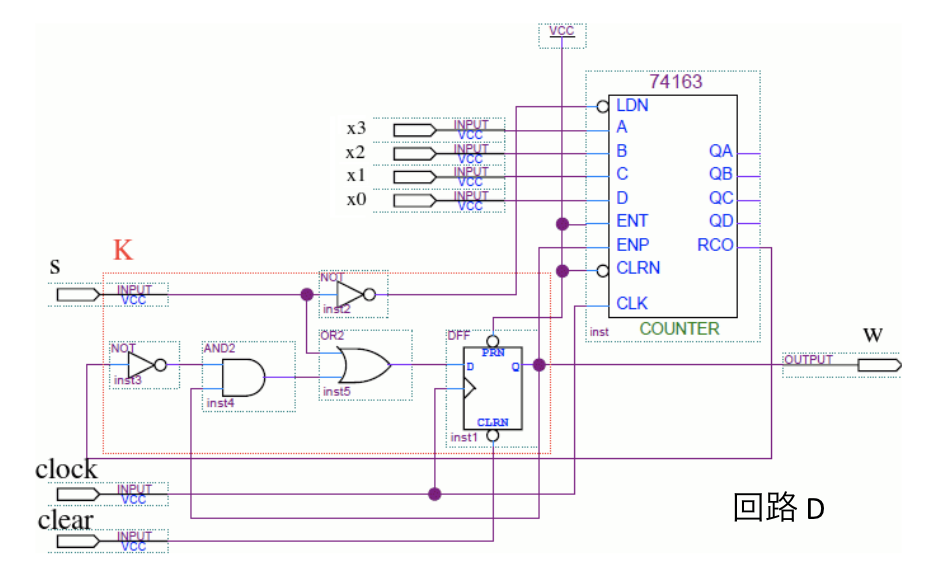
\includegraphics[width=\columnwidth]{asset/ex6_got.png}
	\caption{問題6で与えられた回路図}
	\label{fig:ex6}
\end{figure}

この回路Dは,以下のように動作する.
\begin{quote}
	時刻 $t $にスタート信号 $s$ が $1$ になるとその時刻の $4$ ビットの入力 $x = x_3 x_2 x_1 x_0$ を受け取り,時刻 $t+1$ から $x$ で決まる時間 u$(x) $の間,出力を 1 にする.
\end{quote}

また,回路D内の制御回路Kは,以下のように動作する.

\begin{quote}
	$K1$: $s が 0$ の間待つ.$s が 1$ になると $q' = x$  として $K2$ に進む.	 \\
	$K2$: $q \neq 15$ である間 $q' = q + 1$ を行なうと同時に $w から 1$ を出力.次に,もし $q = 15$ ならば $K1$ へ,さもなければ $K2$ に進む.
\end{quote}


\subsection{原理・理論}

制御回路Kの動作原理より,$s = 1$となったとき$K1からK2$に移行し,$q'$は$x$の入力値を初期値として,1クロックごとに1ずつ増加する.
そして,$q = 15$となったときに$K1$に戻るので,$u(x)$は$x$の入力値によって決まる時間だけ$w = 1$となる.
その具体的な時間は,\ref{eq:ex6}のように与えることができる.

\begin{equation}
	\label{eq:ex6}
	u(x) = 15 - x
\end{equation}

\subsection{回路のアルゴリズム・設計}
\ref{eq:ex6}を実際に確かめるために,$x_0 \sim x_3$の入力を変化させながら32クロック周期のクロック信号を
入力する回路を\ref{fig:ex6-img}のように作成した.

\begin{figure}[htbp]
	\centering
	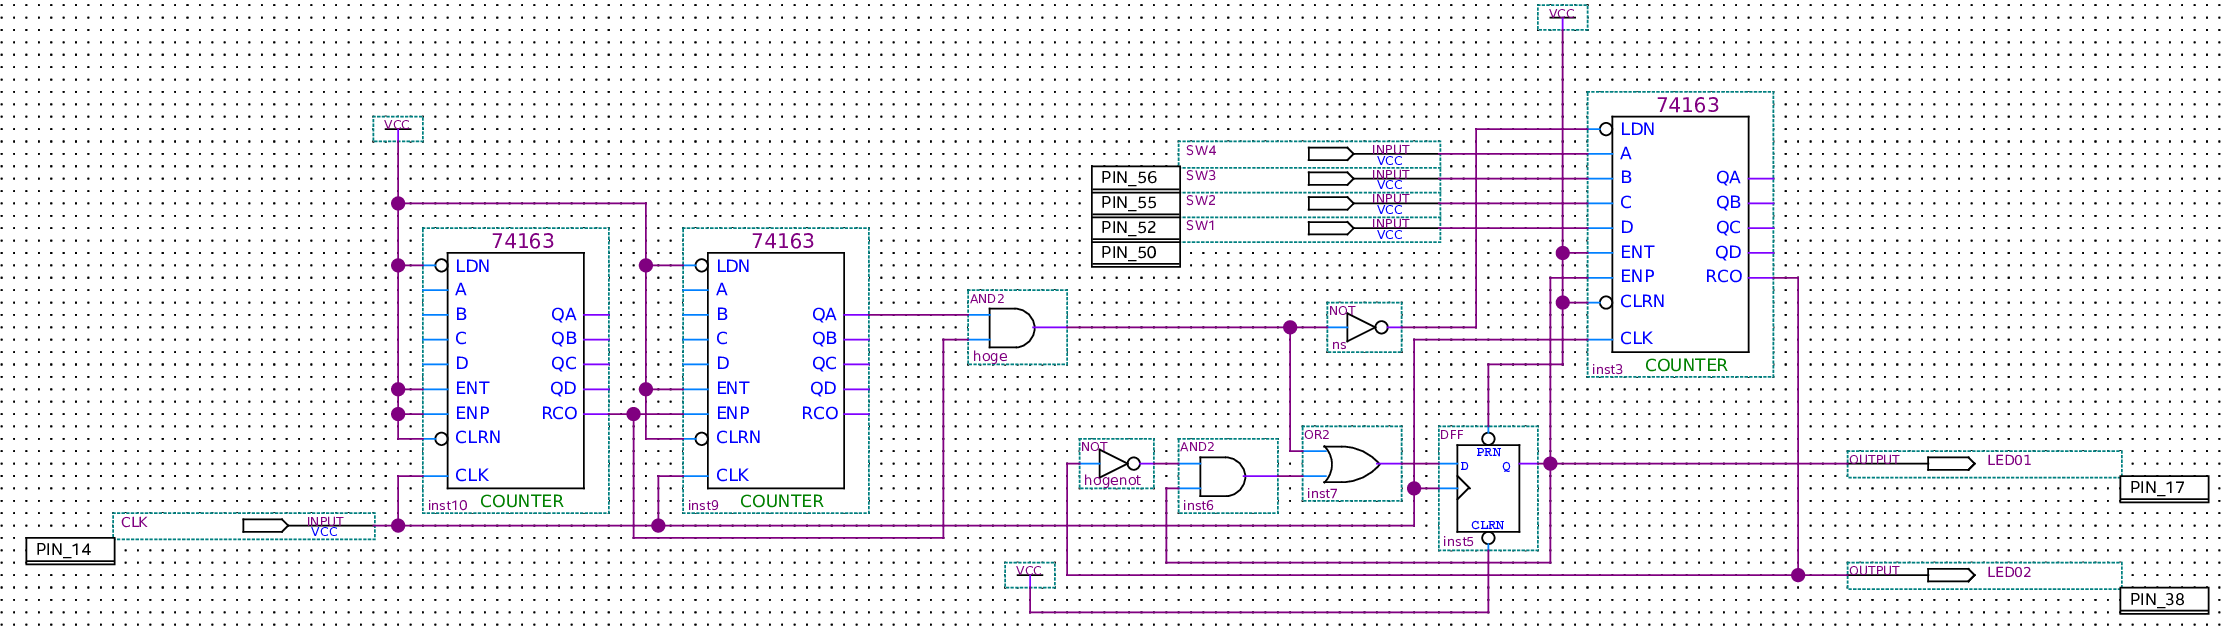
\includegraphics[width=\columnwidth]{asset/ex6a.png}
	\caption{問題6aで使用した回路}
	\label{fig:ex6-img}
\end{figure}

この回路は,$w$と4ビットカウンタのRCO(カウントが0,0,0,0に戻ったときに1になる信号)をLEDに出力するものである.

\subsection{実験・測定結果}

この回路の出力をオシロスコープで観測したところ,\ref{fig:ex6-osc-0},\ref{fig:ex6-osc-8},\ref{fig:ex6-osc-15}のような波形が得られた.
なお,これらの波形では黄色が$w$の出力,紫色が4ビットカウンタのRCO信号である.

波形から,$x$を大きくするほど$w = 1$となる時間が短くなり,$x = 15$を入力した際は$u(x) = 0$となるため$w = 1$となる時間が最も短くなり,
1クロックだけ$w = 1$が出力されていることが確認できた.



\begin{figure}[H]
	\centering
	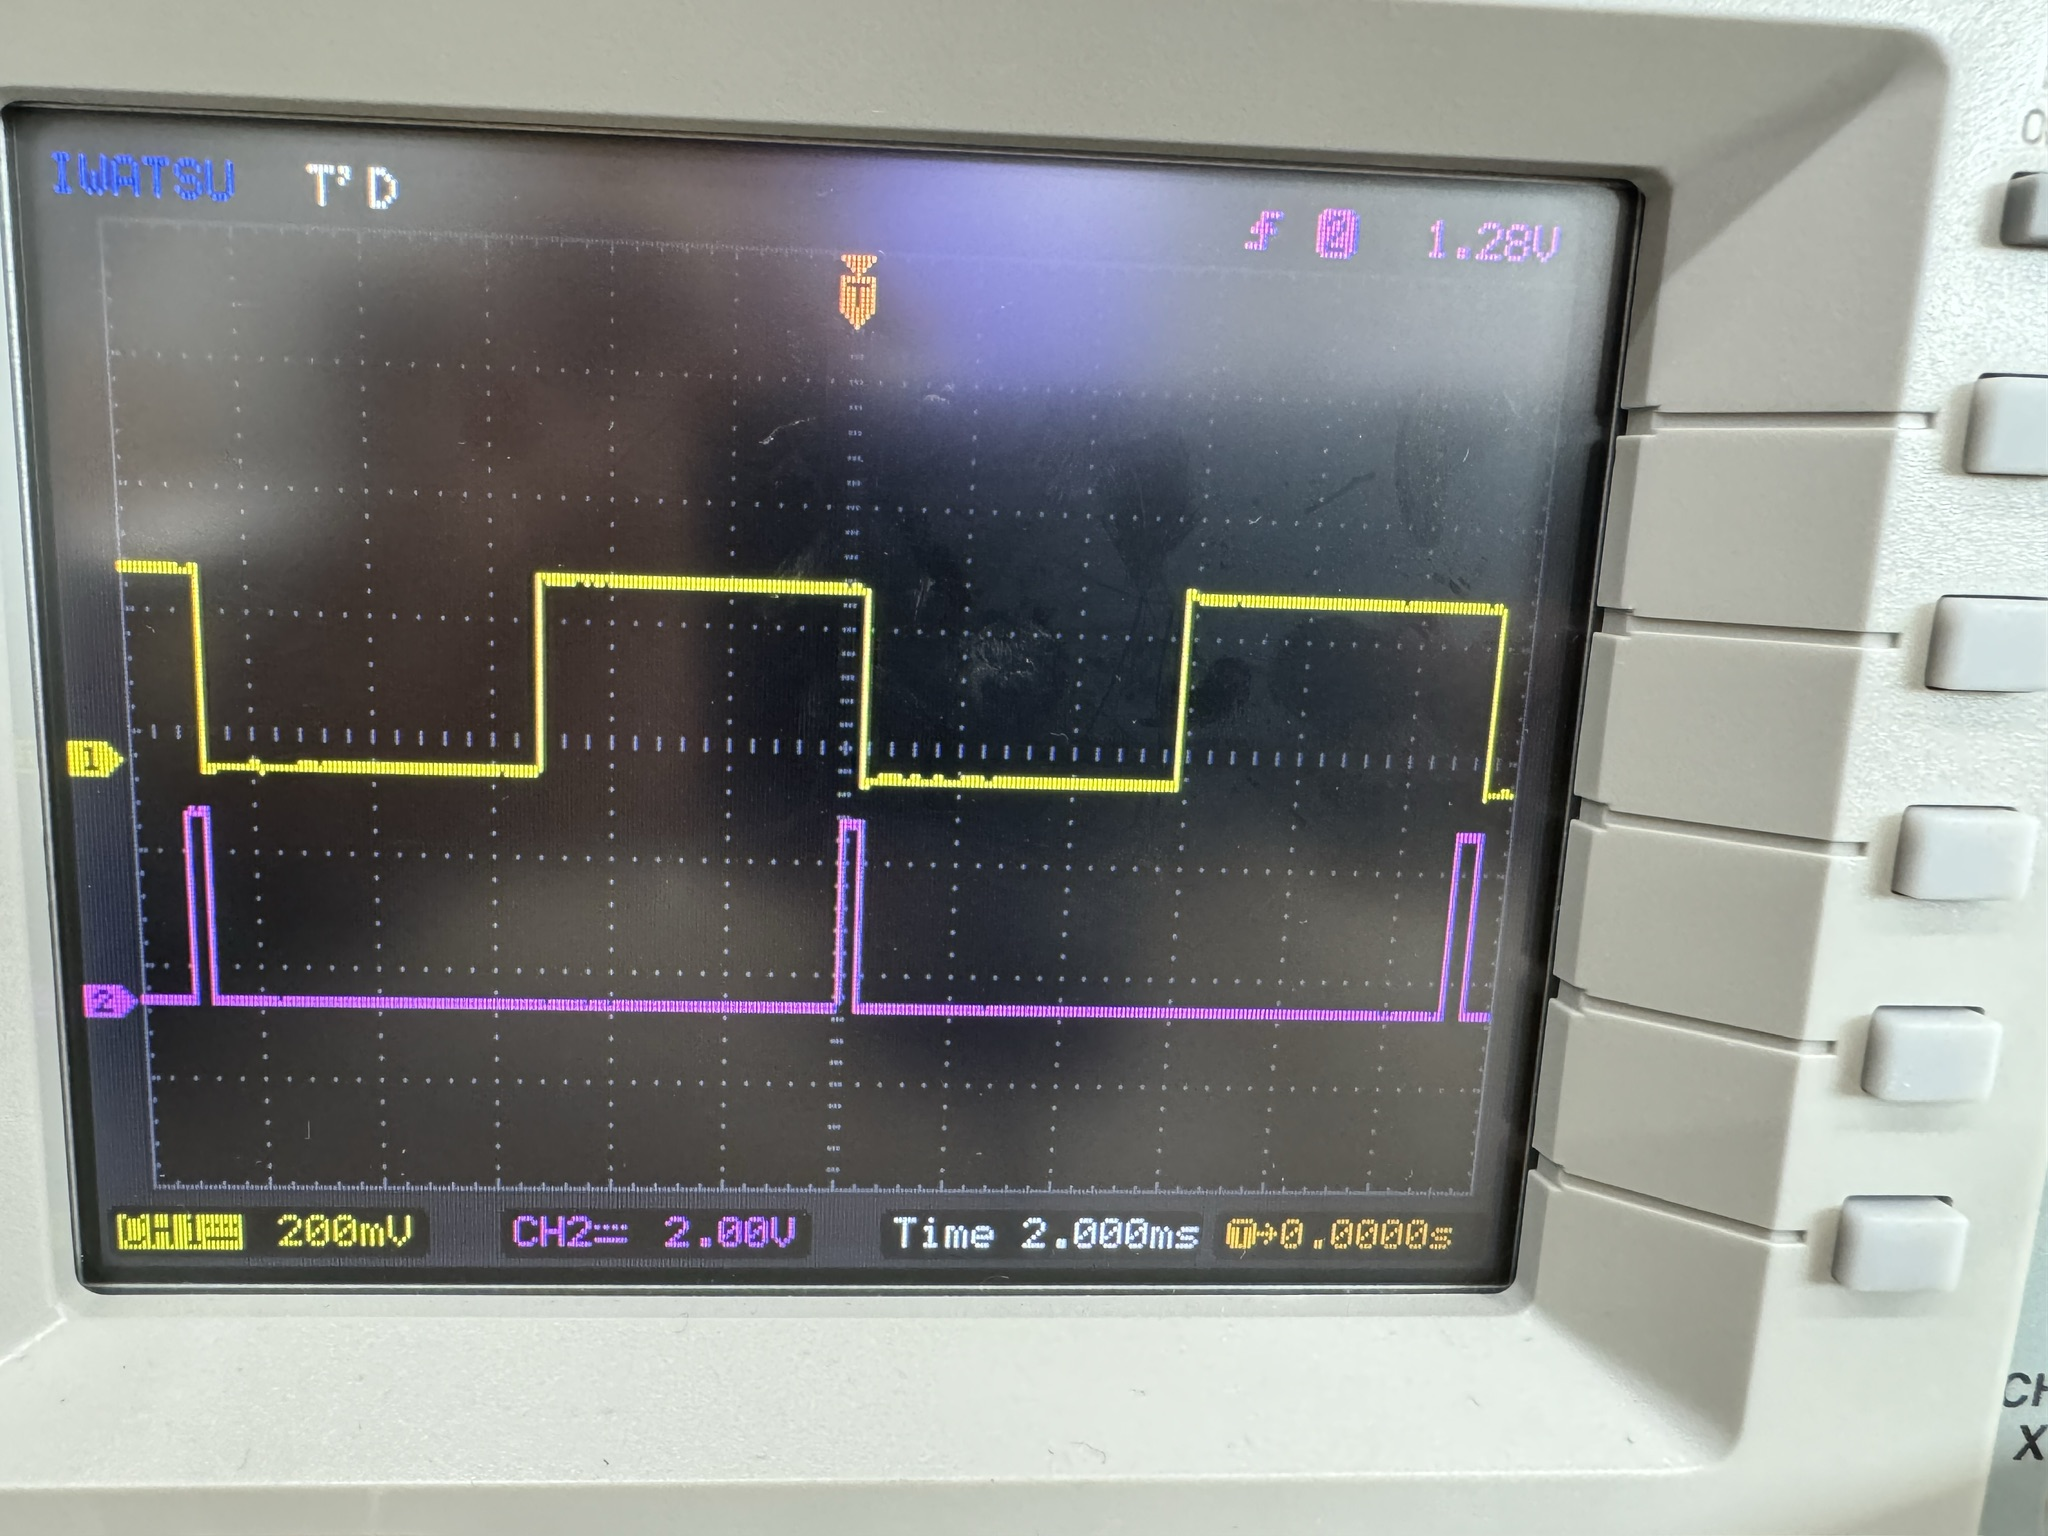
\includegraphics[width=0.8\columnwidth]{asset/ex6a_x_0.jpeg}
	\caption{$x = 0$のときの波形}
	\label{fig:ex6-osc-0}
\end{figure}

\begin{figure}[H]
	\centering
	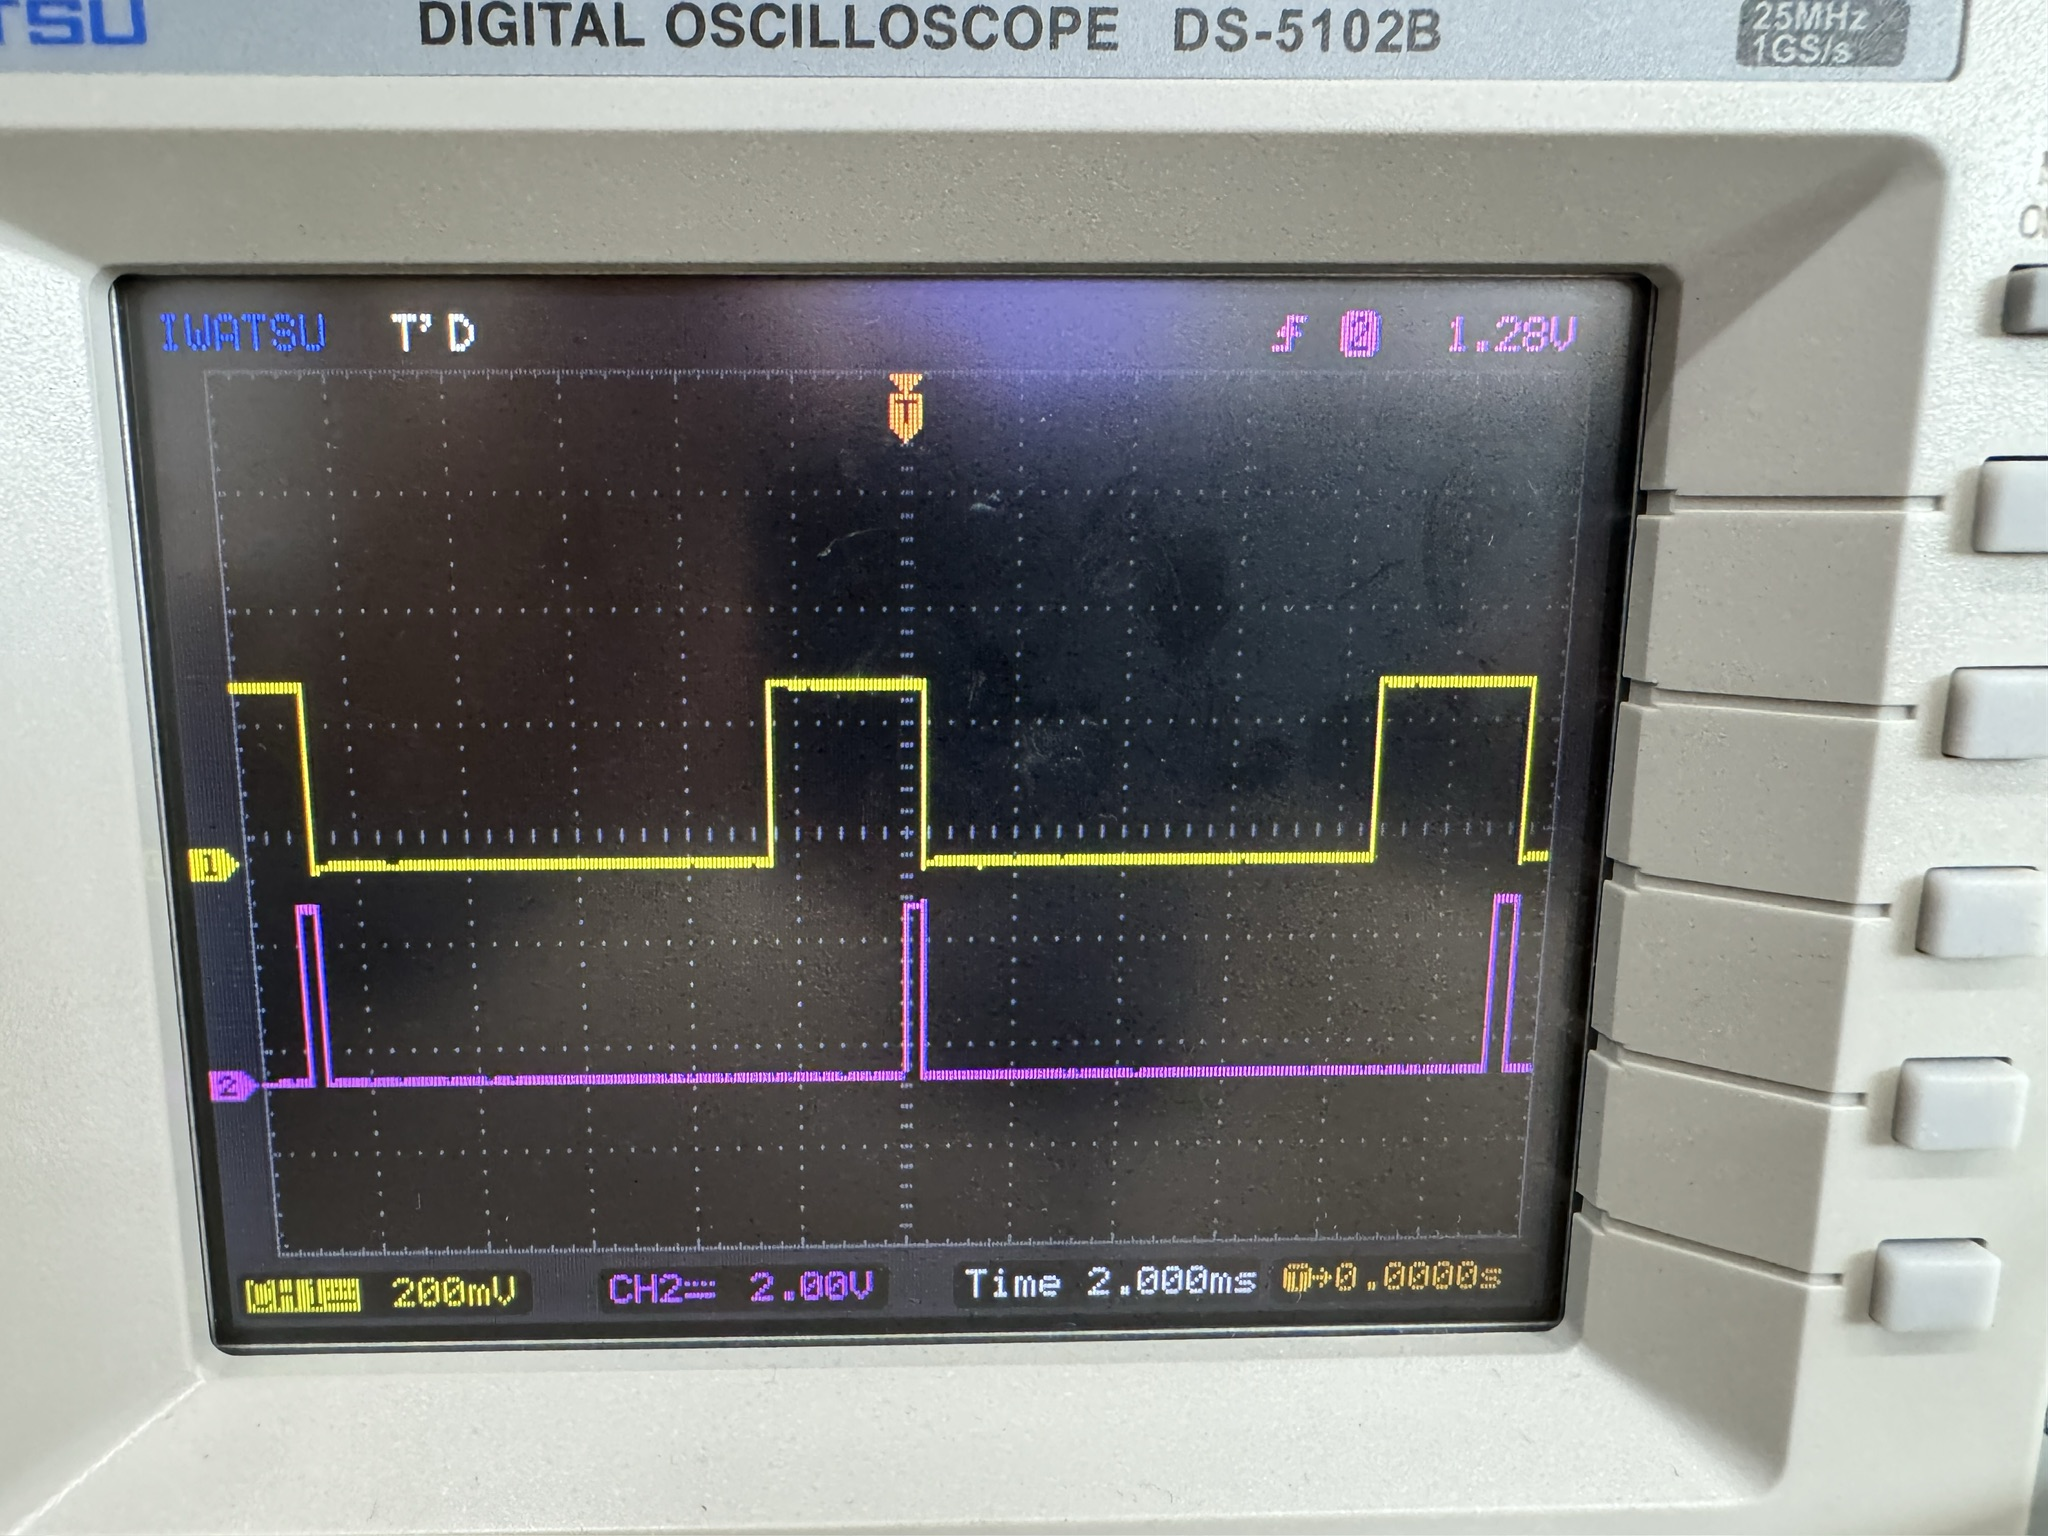
\includegraphics[width=0.8\columnwidth]{asset/ex6a_x_8.jpeg}
	\caption{$x = 8$のときの波形}
	\label{fig:ex6-osc-8}
\end{figure}
\begin{figure}[H]
	\centering
	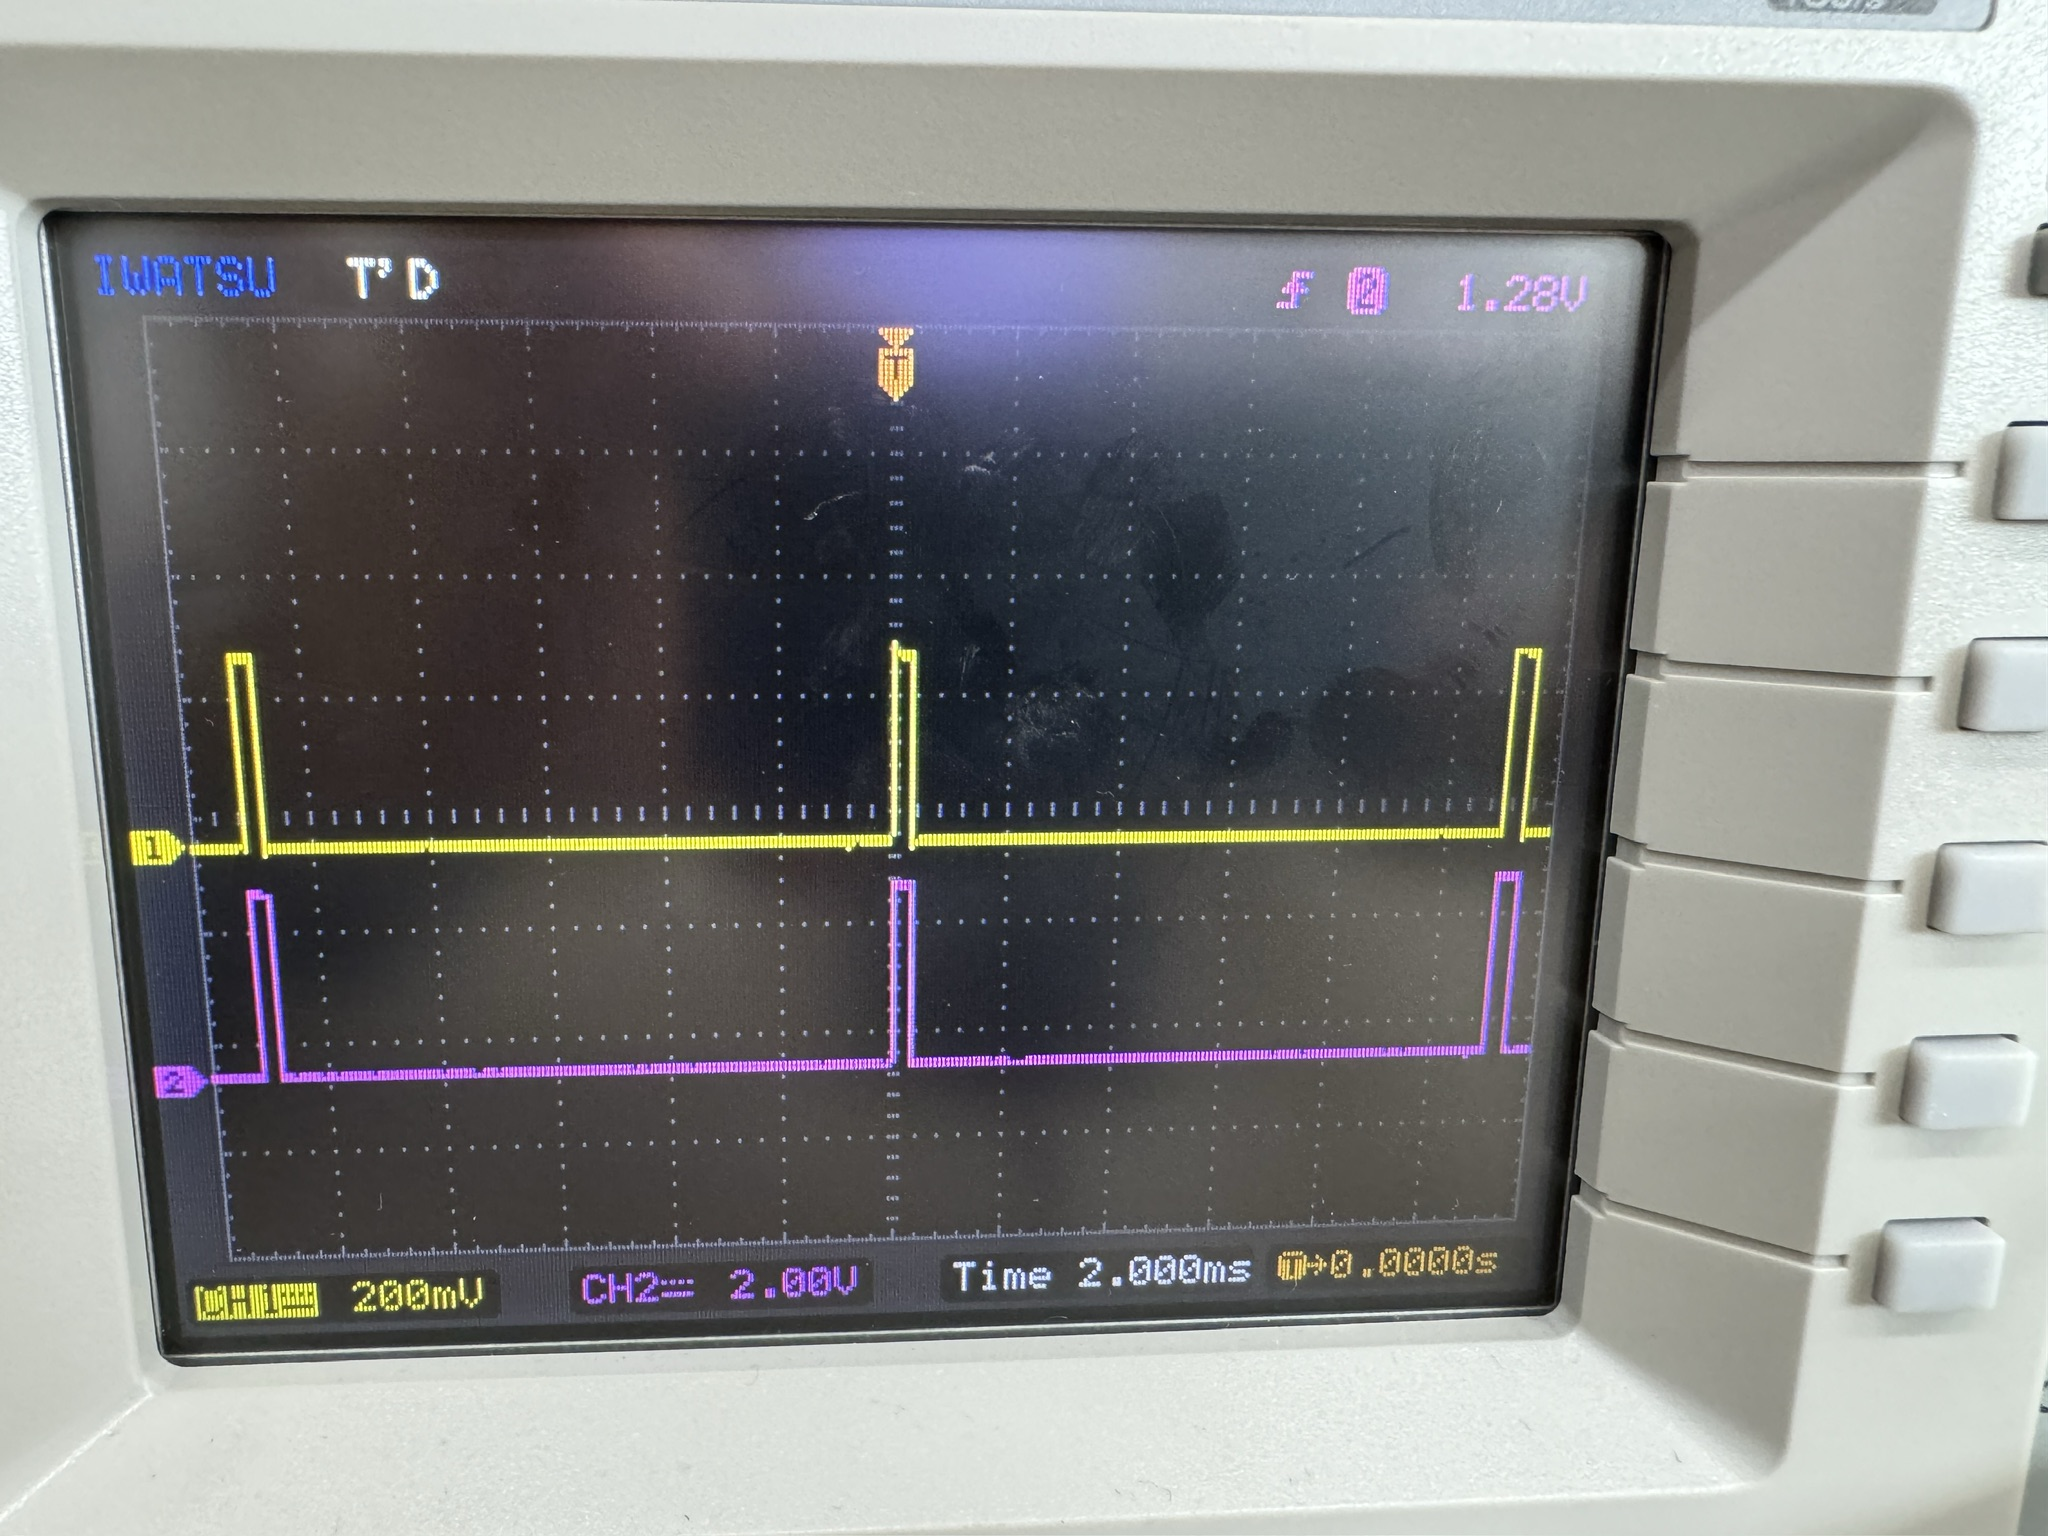
\includegraphics[width=0.8\columnwidth]{asset/ex6a_x_15.jpeg}
	\caption{$x = 15$のときの波形}
	\label{fig:ex6-osc-15}
\end{figure}

\subsection{考察}
また,$x = 0$の際は,$u(x) = 15$となり,$w = 1$が出力される時間が16クロックになるので,
入力$s$の周期を16クロックにしてしまうと$w$がずっと1になってしまう.
このようになると,回路が正しく動作しているか確認できなくなってしまうため,
入力クロックの周期を32クロックに設定していると考えられる.

\section{問題6b}

\subsection{目的}
本問では,\ref{sec:ex6a}の回路Dをもとに,$t$にスタート信号$s$が1になると,その時刻の4ビットの入力
$x = x_3 x_2 x_1 x_0$を受け取り,時刻$t+1$から$t+x$まで出力$w$を1に,
$t + x + 1$に$v$を1にする回路を設計し,その動作を確認する.

\subsection{回路のアルゴリズム・設計}

この問題では,時刻$t + 1$から$t + x$の間で$w = 1$となるので,
$x$クロックの間$w = 1$となるような回路を設計する必要がある.

まず,回路の制御部分を変えずに$x$クロックを測る方法を考える.\ref{sec:ex6a}において
$u(x) = 15 - x$であったが,1の補数の性質に着目すると$u(x) = \bar{x}$となっていることがわかる.

よって,$x$クロックを測るためには,入力$X$を反転させたものを入力として与えればよい.
つまり,$x_0 \sim x_3$をすべてNOTゲートで反転させたものを入力すればよい.

このような$x$を入力すると,$w = 1$となる時間は$x + 1$クロックとなる.
$t$の$x + 1$クロック後は$t + x + 1$であるが,問より$t + x + 1$のとき$v = 1$が出力されていることがわかる.
よって,このときのみ$w = 1$かつ$v = 1$となっている.
なお,$v$は4ビットカウンタのRCO信号を指している.

よって,$w = 1$かつ$v = 1$のときのみ$w = 0$を出力するようにすれば,$x$クロックの間$w = 1$を出力できると考えられる.
このような出力は,$w' = w \oplus v$として$w'$を出力することで実現できる.

\subsection{実際に設計した回路}

これらの考察を踏まえて,\ref{fig:ex6b}のような回路を設計した.

\begin{figure}[htbp]
	\centering
	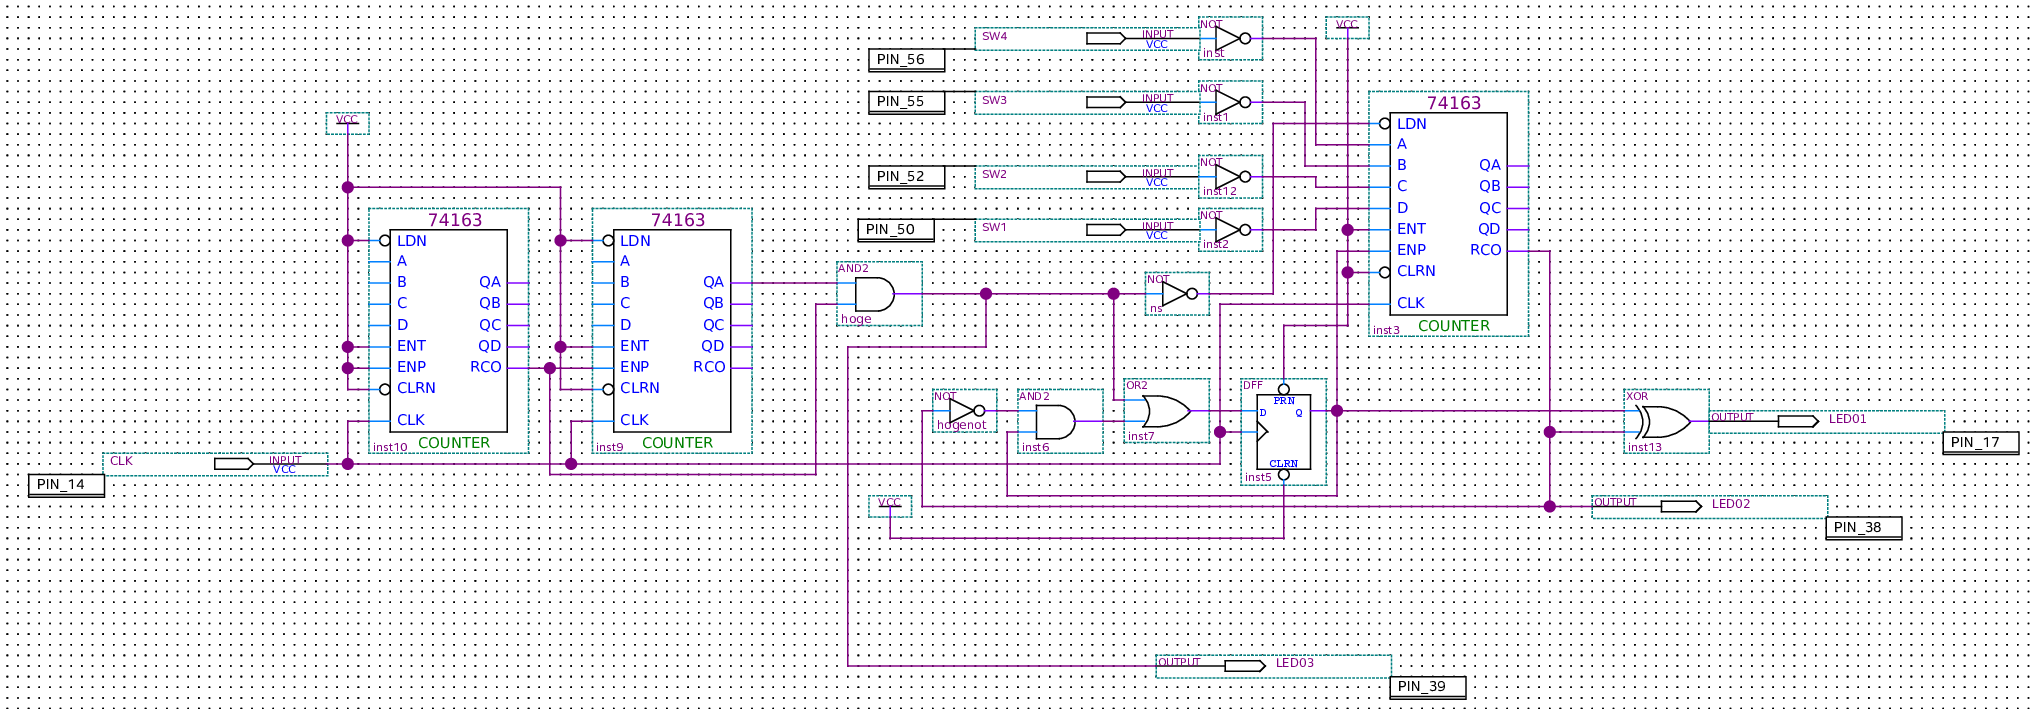
\includegraphics[width=\columnwidth]{asset/ex6b.png}
	\caption{問題6bで設計した回路}
	\label{fig:ex6b}
\end{figure}

\subsection{実験・測定結果}
この回路の出力をオシロスコープで観測した.その際,
トリガとする信号は$s$に設定した.
まず,$w$の波形をオシロスコープで記録し,次に$v$の波形を表示した状態で
記録していた$w$の波形を重ねた.

その結果は\ref{fig:ex6b-osc-0},\ref{fig:ex6b-osc-8},\ref{fig:ex6b-osc-15}のようになった.
白色が$w$, 黄色が$v$, 紫色が$s$である.

\begin{figure}[H]
	\centering
	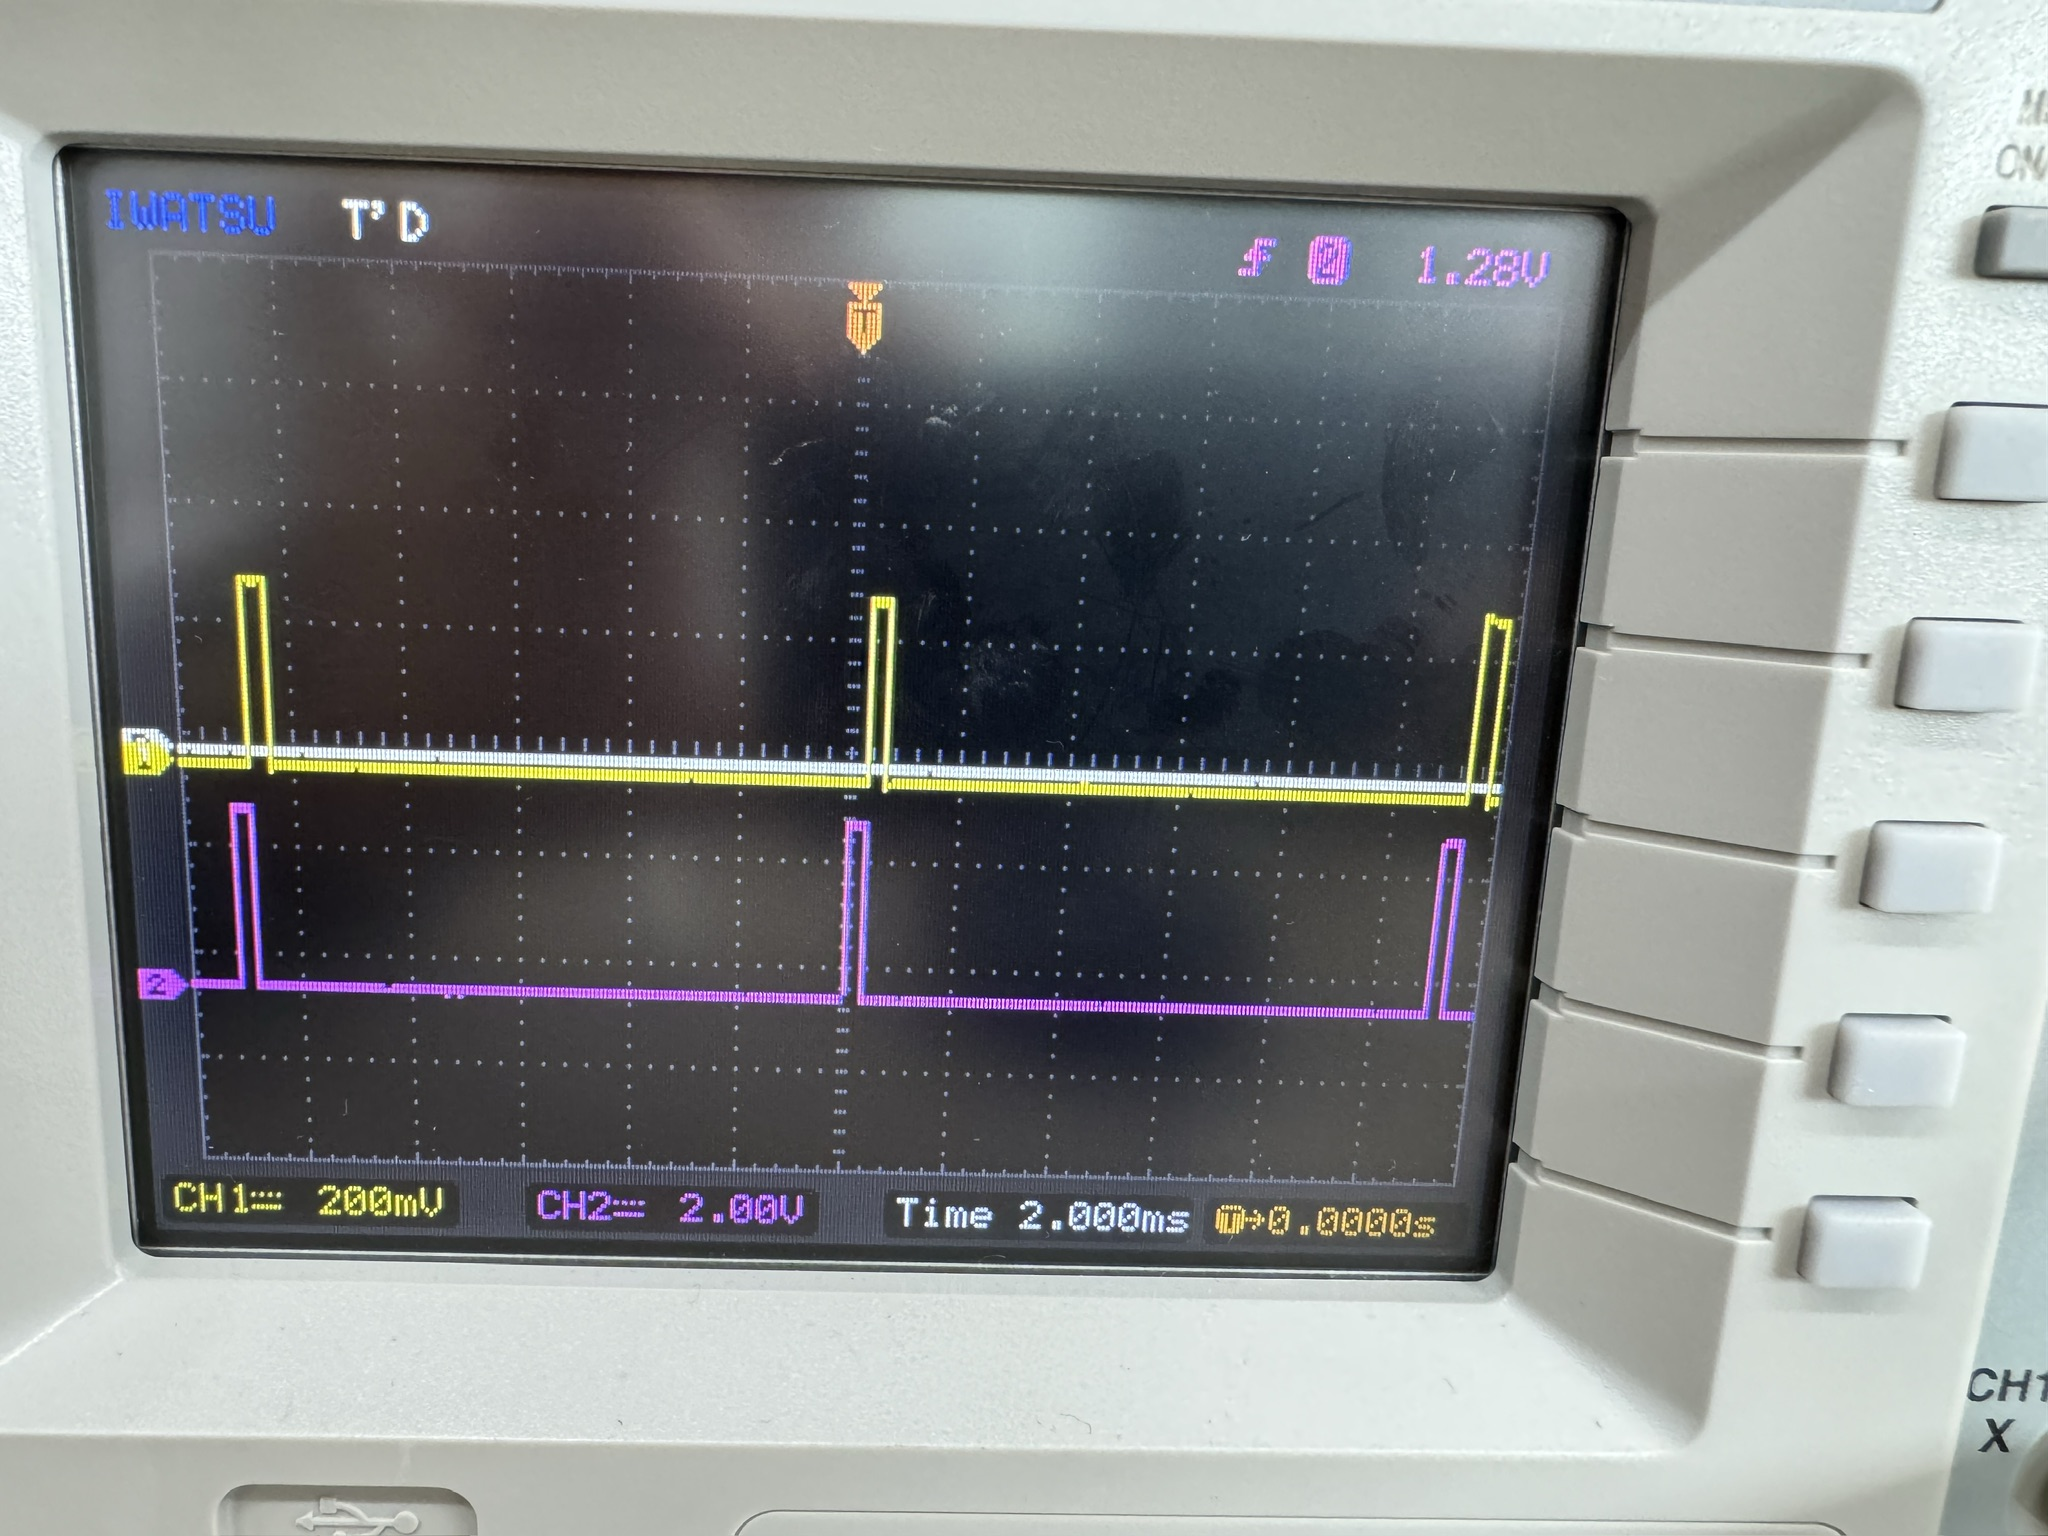
\includegraphics[width=0.8\columnwidth]{asset/ex6b_x_0.jpeg}
	\caption{$x = 0$のときの波形}
	\label{fig:ex6b-osc-0}
\end{figure}

\begin{figure}[H]
	\centering
	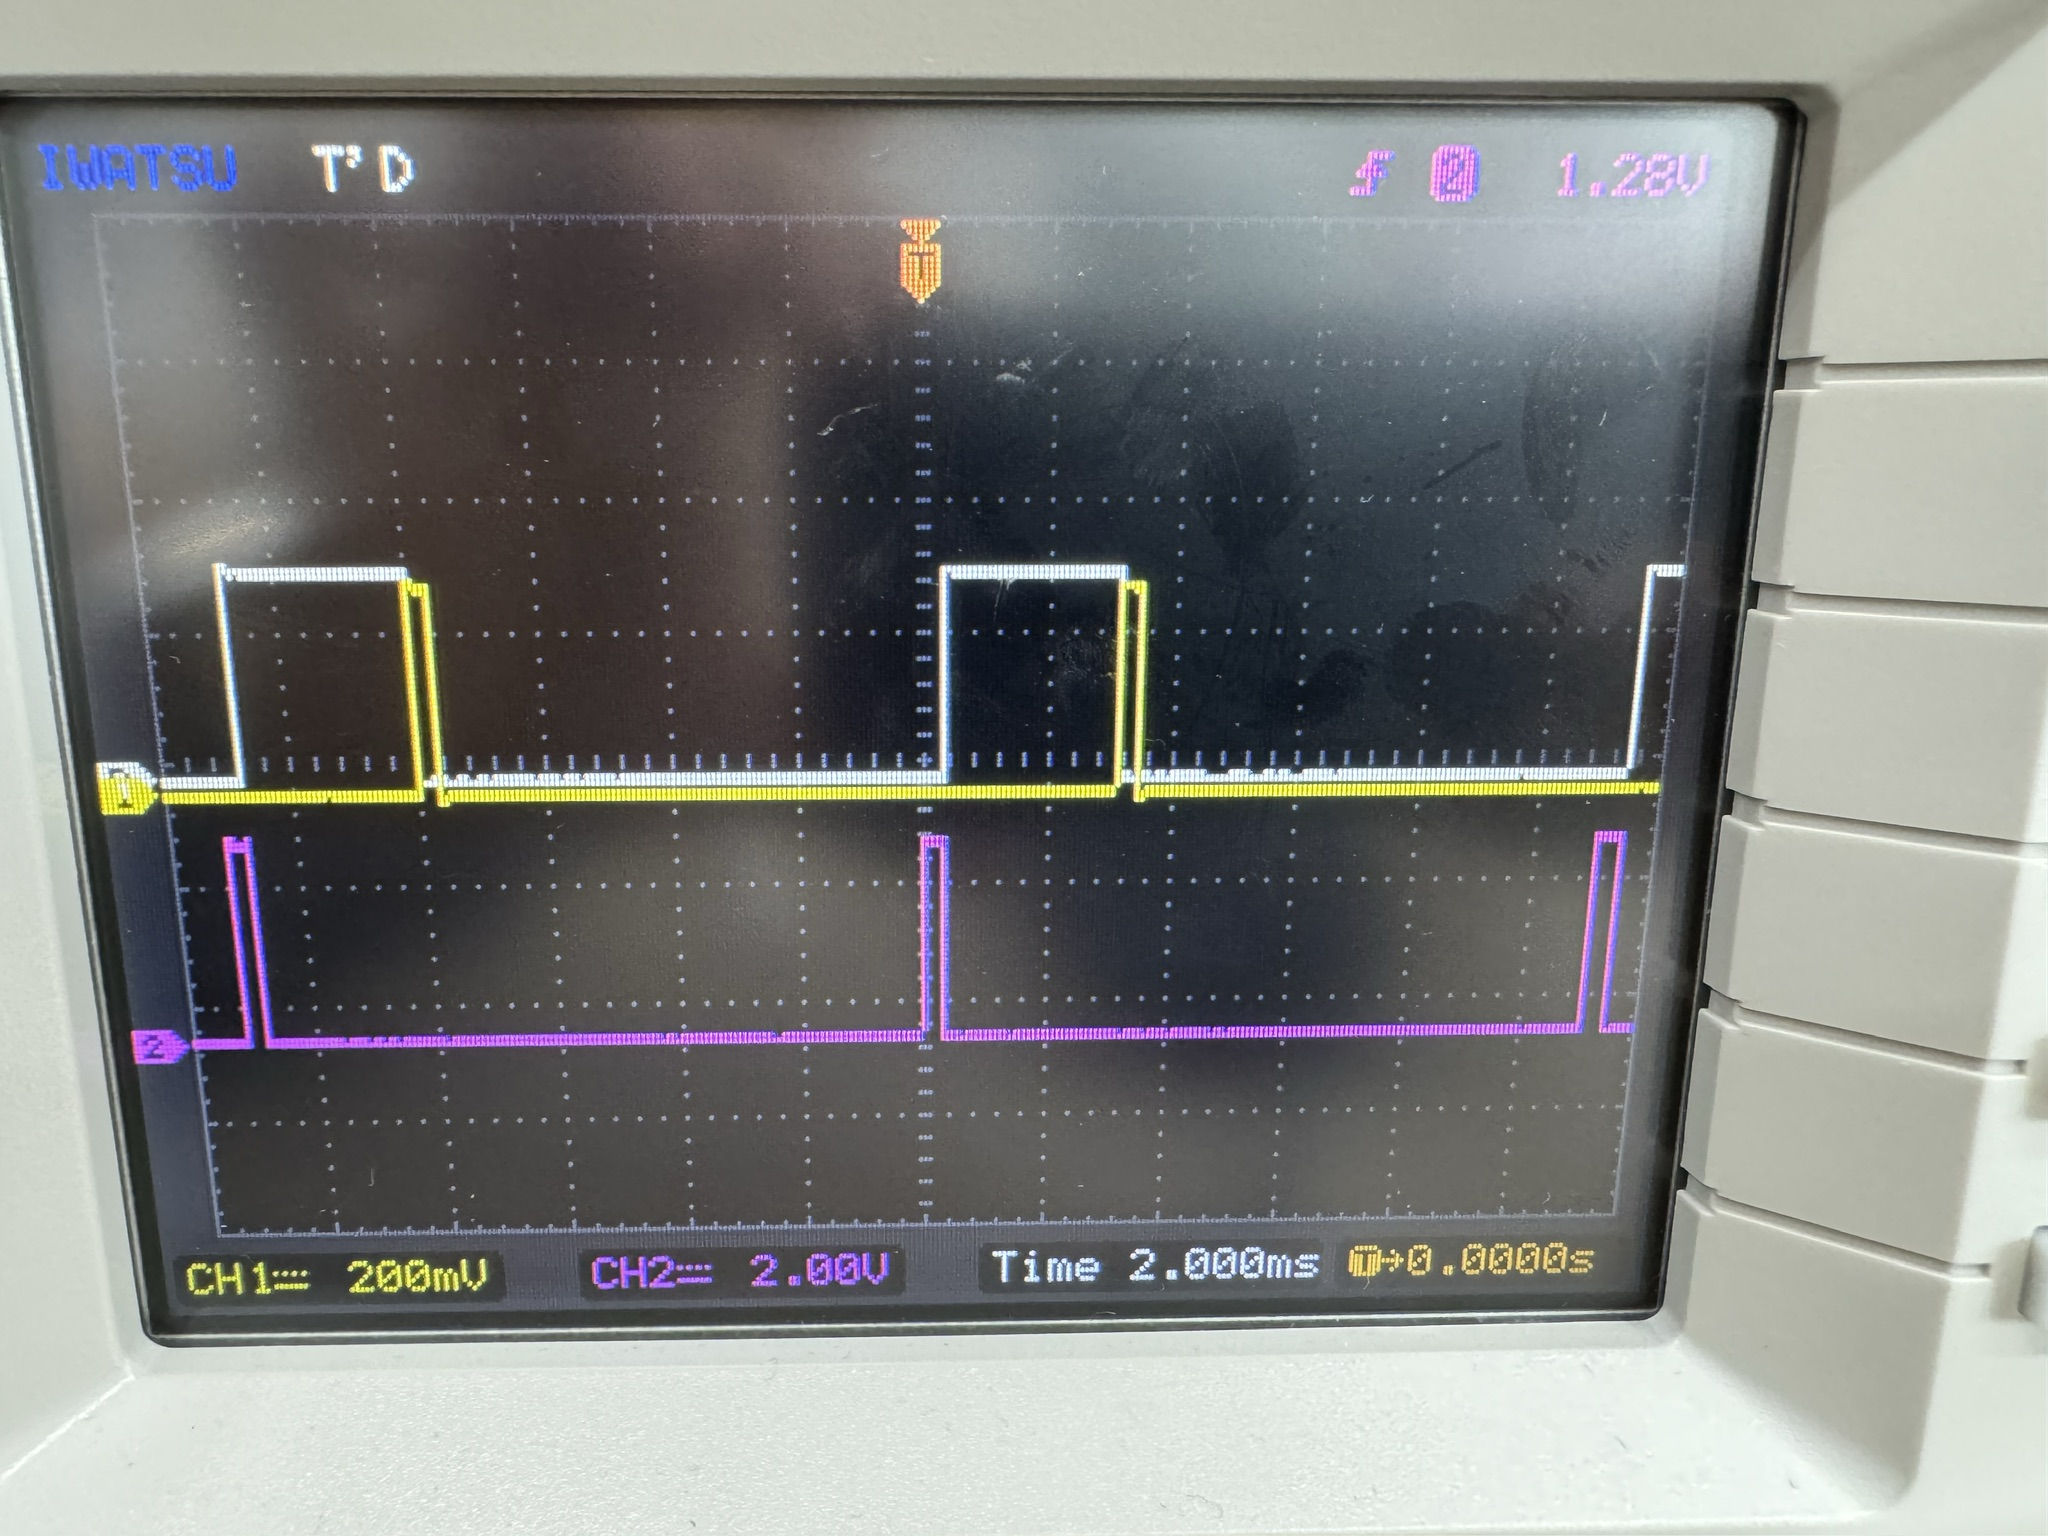
\includegraphics[width=0.8\columnwidth]{asset/ex6b_x_8.jpeg}
	\caption{$x = 8$のときの波形}
	\label{fig:ex6b-osc-8}
\end{figure}

\begin{figure}[H]
	\centering
	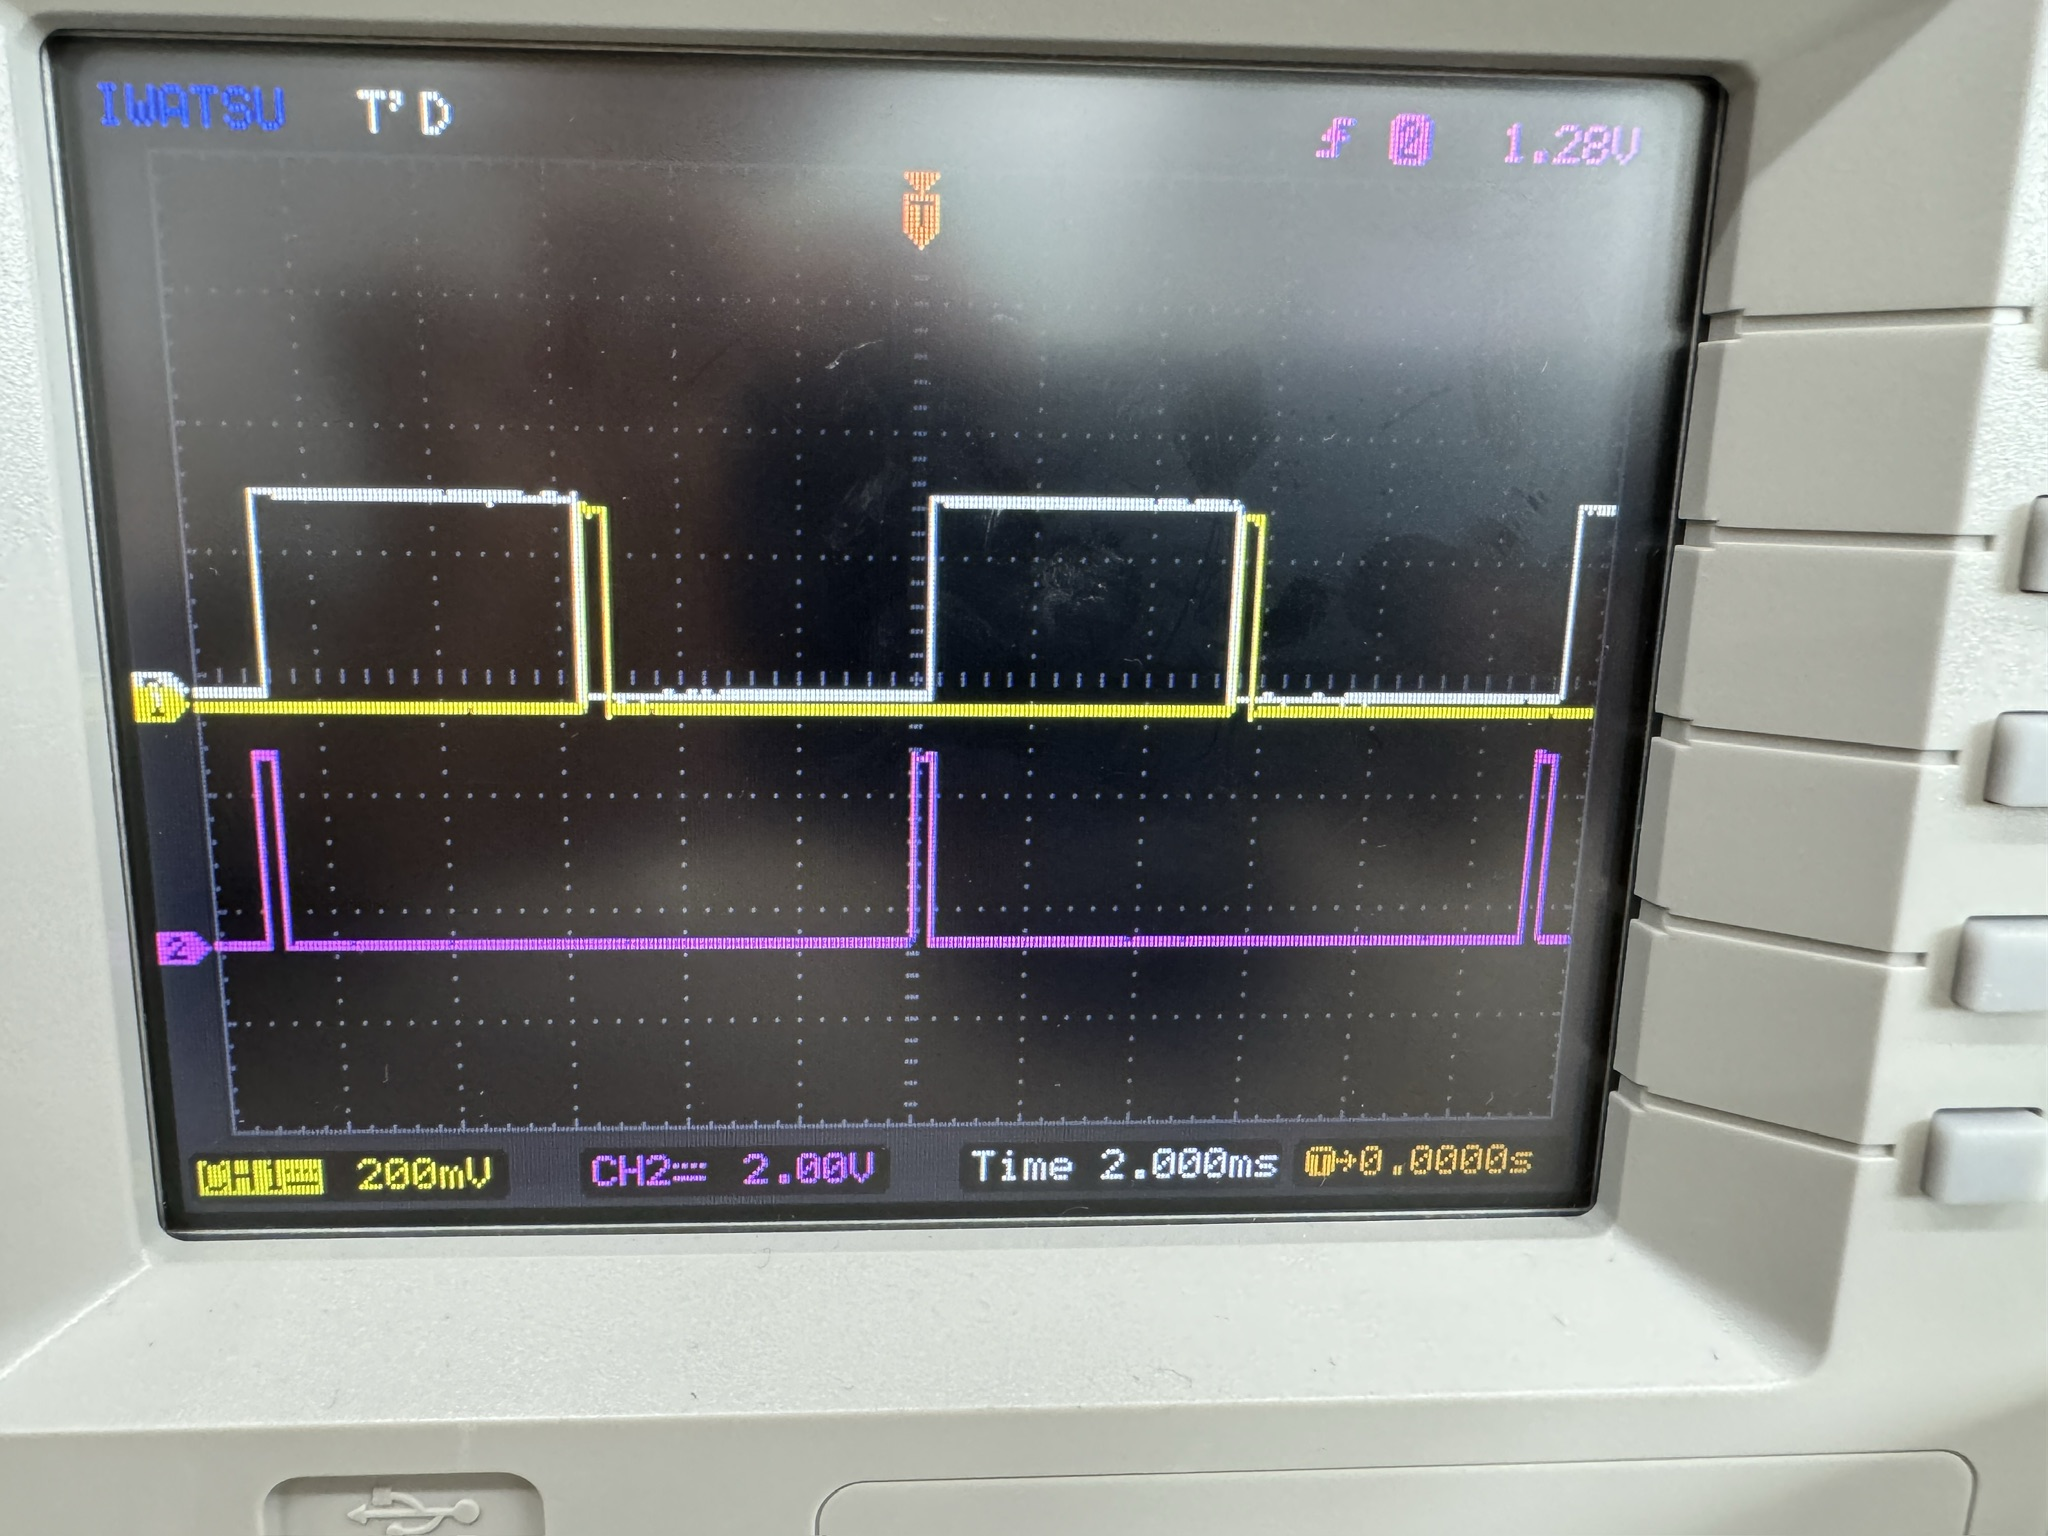
\includegraphics[width=0.8\columnwidth]{asset/ex6b_x_15.jpeg}
	\caption{$x = 15$のときの波形}
	\label{fig:ex6b-osc-15}
\end{figure}

$s = 1$となった次のクロックから$x$クロックの間$w = 1$となり,$w = 0$となった次のクロックで
$v = 1$となることが確認できた.また,$x = 0$のときは$w = 1$となる時間が0クロックであることが確認できた.

よって,問の条件を満たす回路を設計できたと考えられる.

\subsection{考察}
制御部分に手を加えずに,回路の挙動や出力を変化させることができた.
$w = 1$かつ$v = 1$のときだけ$w = 0$を出力するという方法はやや無理やりな方法であると感じたが,
回路の入出力の条件としては正しいので,このような方法もあるということを学ぶことができた.

\end{document}
